% Temporal Hindsight Learning v1

\documentclass[11pt,a4paper]{article}
\usepackage[utf8]{inputenc}
\usepackage[T1]{fontenc}
\usepackage{lmodern}
\usepackage{hyperref}
\hypersetup{colorlinks=true, linkcolor=blue!70!black, citecolor=blue!70!black, urlcolor=blue!70!black}
\usepackage{xcolor}
\usepackage{booktabs}
\usepackage{amsmath}
\usepackage{amsfonts}
\usepackage{amssymb}
\usepackage{amsthm}
\usepackage{arxiv}
\usepackage{microtype}
\usepackage{tikz}
\usepackage{pgfplots}
\pgfplotsset{compat=1.18}
\usepackage{algorithm}
\usepackage{algorithmic}
\usepackage{framed}
\usepackage{graphicx}
\graphicspath{{experiment/output/figures/}}
\usetikzlibrary{shapes,arrows,positioning,shapes.geometric}

% Custom environment for system prompts
\newenvironment{promptbox}[1]
  {\def\FrameCommand{\fboxsep=8pt\fcolorbox{black}{gray!10}}%
    \MakeFramed {\advance\hsize-\width \FrameRestore}
    \textbf{#1}\par\vspace{3pt}\hrule\vspace{5pt}}
  {\endMakeFramed}

\renewcommand{\headeright}{A Preprint}
\renewcommand{\undertitle}{A Preprint}

\date{April 7, 2026}
\title{Temporal Hindsight Learning:\\[0.3em] Blindness as Teacher, Hindsight as Curriculum}
\author{Henrik Westerberg\\Emergent Wisdom\\\texttt{henrik.westerberg@emergentwisdom.org}}

\begin{document}

\maketitle

\begin{abstract}
Language models are lazy optimizers: if a shortcut to the correct answer exists---retrieval, memorization, pattern matching---the gradient will reinforce it over the harder path of causal reasoning. We observe that the knowledge cutoff, normally treated as a deficiency of LLMs, is one mechanism that reliably blocks this shortcut. When the outcome is strictly masked, the only path to low loss is reasoning. Blindness is the teacher.

We present Temporal Hindsight Learning (THL), which engineers this observation into a training framework. By deliberately stacking models at distinct temporal positions (a past-frozen Student blind to outcomes, a temporally advantaged Teacher with hindsight, and an independent Auditor), THL converts the knowledge cutoff from a passive limitation into the primary instrument that forces reasoning over retrieval. The Teacher, knowing how events unfolded, works backward to identify the causal signals that were available before the outcome---generating structured reasoning supervision that the Student, constrained to the past, must derive rather than retrieve.

We introduce a five-angle causal decomposition (the Forecasting Pentagon) and a formal leakage-detection protocol (the Erasure Test). In a small-scale pilot study training on 106 events from 2024 ($N=505$ traces across five reasoning angles) and evaluating on 15 unseen 2025 events, a 70B THL Student improves reasoning quality by 20\% over its base model ($p < 0.001$) and approaches the frontier Teacher in prediction accuracy. These preliminary results suggest that for open-ended reasoning, the quality of supervision may matter more than the scale of the model.
\end{abstract}

%==============================================================================
\section{Introduction}
%==============================================================================

Neural networks are lazy optimizers. Given a path through retrieval and a path through reasoning, the gradient will reinforce whichever minimizes loss more cheaply---and retrieval is almost always cheaper. Standard training exacerbates this: when the model's training data covers an event, the loss can be minimized by memorizing the token sequence of the outcome, and the gradient reinforces storage circuits. The result is models that can retrieve ``Trump wins 2024'' without any structural understanding of why. These are Almanac-readers, not Analysts.

But when the outcome is strictly masked---when the knowledge cutoff falls before the event---the retrieval shortcut vanishes. The only path to low loss is to identify the latent causal bridge between available evidence and the target. The gradient has no choice: it must reinforce logic circuits. The knowledge cutoff, normally treated as a deficiency of LLMs, is the one mechanism that forces reasoning over retrieval. \textbf{Blindness is the teacher.}

Blindness alone, however, produces only failure. A model blind to outcomes with no guidance will simply predict badly. The critical complement is structured hindsight. A Teacher model with knowledge of how events unfolded can trivially work backward to identify the causal signals that were available before the outcome. This exploits a deep asymmetry: identifying the ``smoking gun'' after the crime is easy; spotting it in real-time noise is exactly the hard skill. THL pairs engineered blindness with structured hindsight: the Teacher generates the curriculum, and the Student's blindness ensures it must reason through it rather than memorize it. \textbf{Hindsight is the curriculum.}

This framework contributes to an emerging paradigm we call \emph{Supervision by Reality}. Current reasoning research relies on Supervision by Compiler (math and code, where correctness is deterministic) or Supervision by Proxy (human preference labels, which are expensive and gameable). THL explores a third mode: using the passage of time as an objective, ungameable verifier for open-ended causal reasoning. Compilers check syntax; humans check style; the future checks causality. While binary prediction markets have been used as outcome-supervised training signals~\cite{turtel2025selfteach, turtel2025rlvr, turtel2026futureaslabel}, THL targets the harder problem of open-ended causal reasoning, requiring a fundamentally different architecture. Our contribution is the recognition that the knowledge cutoff is not merely a source of labels but a \emph{controllable instrument for forcing reasoning}: (1)~cross-family temporal distillation where the Teacher's advantage is temporal, not capacity-based; (2)~the Forecasting Pentagon, a five-angle causal decomposition that generates structured multi-angle training signal from each event; (3)~the Erasure Test, a formal leakage-detection protocol; and (4)~the Council of Time, a theoretical blueprint for converting the entire historical record into a chronological reasoning curriculum.

The framework relies on engineered temporal gaps (Figure~\ref{fig:temporal-gap}). We deliberately stack three models with different knowledge cutoffs (Llama at Dec 2023, Gemini at Jan 2025, Claude at May 2025) so that each plays a distinct temporal role: the Student is frozen in the past, the Teacher has hindsight over the training period, and the Auditor has hindsight over the test period. The Teacher, with access to events at time $t$, acts as a causal detective: it analyzes the outcome to identify the specific ``smoking gun'' clues that were available at $t-\Delta$, then generates a research dossier framed through the Forecasting Pentagon (Section~\ref{sec:pentagon}). The Student, constrained to data prior to $t$, receives these clues and must generate a context-injected chain-of-thought, explicitly separating pre-training knowledge from the new context before deriving a calibrated prediction.

\begin{figure}[htbp]
\centering
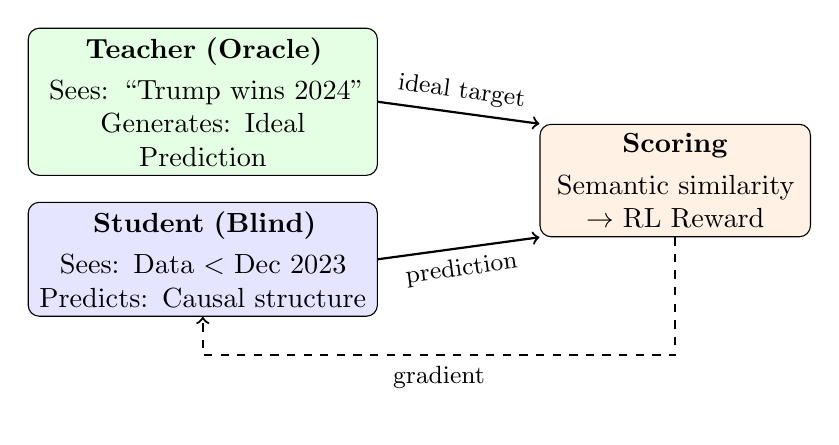
\begin{tikzpicture}[node distance=1.5cm]
\node[draw, rounded corners, fill=green!10, text width=4.2cm, align=center] (teacher) at (0,2) {
    \textbf{Teacher (Oracle)}\\[0.3em]
    Sees: ``Trump wins 2024''\\
    Generates: Ideal Prediction
};
\node[draw, rounded corners, fill=blue!10, text width=4.2cm, align=center] (student) at (0,0) {
    \textbf{Student (Blind)}\\[0.3em]
    Sees: Data $<$ Dec 2023\\
    Predicts: Causal structure
};
\node[draw, rounded corners, fill=orange!10, text width=3.2cm, align=center] (score) at (6,1) {
    \textbf{Scoring}\\[0.3em]
    Semantic similarity\\
    $\rightarrow$ RL Reward
};

\draw[->, thick] (teacher.east) -- node[above, sloped, font=\small] {ideal target} (score.north west);
\draw[->, thick] (student.east) -- node[below, sloped, font=\small] {prediction} (score.south west);
\draw[->, thick, dashed] (score.south) -- ++(0,-1.5) -| node[pos=0.25, below, font=\small] {gradient} (student.south);
\path (0,-2); % extend bounding box
\end{tikzpicture}
\caption{The Teacher-Student temporal gap. The Teacher (with hindsight) generates a Research Dossier with context clues; the Student (blind to the future) must derive a prediction via Chain-of-Thought. The scoring function validates the causal bridge.}
\label{fig:temporal-gap}
\end{figure}

Why does hindsight improve foresight? We posit that standard pre-training fails because the signal-to-noise ratio in raw history is too low. In January 2024, the signal ``loose bolts found on United Airlines flights'' was buried under thousands of noise tokens (fuel targets, labor disputes, stock buybacks).

THL creates a Teacher-Author / Student-Detective dynamic. The Teacher, knowing the ending (Boeing Grounded), works backward to identify the ``Smoking Gun'' (the loose bolts) and plants it in the context. The Student, blind to the outcome, is trained to prioritize this specific signal over the noise. By training on thousands of these reverse-engineered mysteries, the Student learns the \textit{pattern} of a smoking gun (e.g., ``Systemic manufacturing escape across multiple units $\approx$ 100\% grounding risk''), allowing it to spot such signals in real-time in the future.

Consider the central plot device of \textit{Back to the Future Part II}: the Sports Almanac. When Old Biff gives Young Biff the book of future scores, Young Biff becomes wealthy but not intelligent. He relies entirely on \textit{retrieval}. If the timeline diverges (e.g., the book is burned), his predictive capability collapses to zero. He is an overfitted model.

THL proposes a different interaction. Imagine Old Biff is forbidden from transferring the book (The Facts) but is allowed to become a Tutor. He cannot say ``The Dodgers win in 1955.'' Instead, he uses his hindsight to teach Young Biff: ``In 1955, pay attention to the Dodgers' late-inning performance against left-handed pitchers. There is a structural anomaly there.'' Young Biff must then observe the context and \textit{deduce} the outcome.

If Young Biff undergoes this training 500 times, he does not just memorize the 1955 season. He learns a generalizable skill: how to analyze baseball statistics. If we then transport him to a year beyond the Almanac's coverage, he will outperform a standard gambler because he has learned the \textit{mechanism} of the game (e.g., the Lefty Pitcher anomaly), not just the specific scores. He has internalized the Oracle's wisdom without needing the Oracle's presence.

\medskip\noindent\textit{Defining the Ideal Cutoff.}
We define the optimal knowledge cutoff $\tau^*$ for a given event $e$ occurring at time $t_e$ as:
\begin{equation}
    \tau^* = t_e - \epsilon
\end{equation}
where $\epsilon$ is the minimal duration required to prevent information leakage. If $\tau \ll t_e$ (e.g., years prior), the model lacks the contextual primitives to interpret the clues---a 2019 model cannot reason about ``Omicron variants.'' Conversely, if $\tau \ge t_e$, the model collapses into retrieval. THL maintains the model in this ``Goldilocks Zone'' of maximum context with zero hindsight, ensuring that high performance can only be achieved through superior causal simulation. In this pilot, $\epsilon \approx 1$ month: the Teacher's knowledge extends through January 2025, and the test events span February--May 2025. The optimal $\epsilon$ is likely domain-dependent (political events may require finer temporal resolution than technological trends), and systematic ablation of this parameter remains future work. This equation governs a single event; at full scale, the same principle applied iteratively across chronological eras yields the \textit{Council of Time} (Section~\ref{sec:council}): a training protocol where the model must predict each decade's structural outcomes before being allowed to read about them, converting the entire pre-training corpus into a sequential reasoning curriculum.

A naive approach would score the student against the literal event (``Trump wins''). This is problematic because it rewards lucky guesses equally with reasoned predictions, provides no gradient (either exact match or nothing), and conflates predictable structure with unpredictable specifics.

The Teacher's role is to generate what good foresight looks like: the reasoning a skilled forecaster would produce. This includes broad strokes that were inferable from past data, appropriate uncertainty about specifics, and calibrated confidence levels.

Consider a 1995 thought experiment where we ask two forecasters about the future of information. \textit{Forecaster A} says: ``A global network will connect everyone, dominated by giant corporate portals harvesting user attention for ad revenue.'' \textit{Forecaster B} says: ``The internet will be a decentralized utopia powered by Netscape Navigator.'' Today, we recognize Forecaster A was structurally correct. Though they missed specific names like ``Google'' or ``Facebook,'' they correctly identified the incentives (consolidation, ad revenue). Forecaster B was specific (``Netscape'') but structurally wrong.

Standard evaluation fails this test. Scored on ``Did they mention Facebook?'', both fail. Scored on ``Did they mention Netscape?'', Forecaster B might win.

THL acts as a fair judge. The Teacher, armed with hindsight, validates Forecaster A's reasoning (``consolidation,'' ``ad revenue''), awarding points because these reasons proved to be the causal drivers. We grade the quality of the justification, not merely the exactitude of the noun.

We validate the technique with a pilot study (Section~\ref{sec:gsr}) training a 70B model on Teacher-generated reasoning traces from 2024 events, then evaluating on unseen 2025 events. The full experimental setup and results are reported in Section~\ref{sec:experiment}.

\medskip\noindent\textbf{Summary of Contributions.}
THL introduces five mechanisms that are, to our knowledge, novel:

\begin{enumerate}
    \item \textbf{Cross-family hindsight distillation.} The Teacher (Gemini) generates ``ideal prediction'' traces using its temporal advantage over the Student (Llama), while an independent Auditor (Claude) from a third model family scores the results. The Teacher's advantage is temporal, not capacity-based, and no model family occupies more than one role.

    \item \textbf{The Forecasting Pentagon.} Each event is analyzed through five complementary reasoning angles (Structural, Economic, Political, Base Rates, Temporal), generating $5\times$ training signal per event and teaching the Student to approach forecasting from multiple analytical frameworks.

    \item \textbf{Engineered temporal gaps.} Three models with different knowledge cutoffs serve strictly separated roles, preventing stylistic alignment from inflating evaluation scores.

    \item \textbf{Post-hoc rationalization as pedagogy.} The training data consists of high-quality post-hoc rationalizations using only pre-cutoff vocabulary---the same mechanism by which case-study pedagogy teaches forecasting in business schools and military academies. We argue this is a feature, not a limitation, and provide evidence that the reasoning strategy transfers to genuinely novel events (Section~\ref{sec:experiment}).

    \item \textbf{The Erasure Test (Specifics Reconstruction Rate).} A formal leakage-detection protocol that feeds the Teacher's reasoning trace into a frozen, cutoff-matched model to measure whether the trace inadvertently encodes future specifics. This provides a quantifiable quality-assurance metric for hindsight-generated training data, addressing the ``Simulated Ignorance'' problem~\cite{li2026simulated} through detection rather than prompt-based mitigation.
\end{enumerate}

%==============================================================================
\section{Related Work}
%==============================================================================

THL synthesizes three research threads: temporal evaluation, capability distillation, and hindsight-based reinforcement learning---and positions itself against a rapidly growing body of concurrent work on outcome-supervised forecasting.

\paragraph{Temporal Evaluation and Forecasting.}
ForecastBench \cite{karger2025forecastbench} evaluates LLMs on prediction markets, while Halawi et al.~\cite{halawi2024forecasting} demonstrated a retrieval-augmented system approaching human crowd accuracy. Mind the Gap \cite{lazaridou2021mind} explores temporal generalization, Time-R1 \cite{timer1_2025} proposes temporal curriculum training via staged RL, and the AIA Forecaster~\cite{aia2025} achieved the first verified expert-level forecasting at scale using multi-agent prompting. We extend these by introducing the Teacher-Oracle mechanism to generate rich \textit{training} targets, not just evaluation metrics or inference-time strategies.

\paragraph{Distillation and Reasoning Supervision.}
While standard distillation transfers capabilities from larger to smaller models \cite{hinton2015distilling}, our Teacher is not necessarily larger---it is \textit{temporally advantaged}, generating structured prediction targets rather than soft labels. Our approach adapts ``Weak-to-Strong Generalization'' \cite{burns2023weaktostrong} to the temporal axis: the teacher doesn't need to be smarter, it just needs to be \textit{later}. DeepSeek-R1~\cite{deepseekr1} demonstrated that distilling reasoning traces from large to small models outperforms direct RL on smaller models, directly motivating our SFT-based approach. Hsieh et al.~\cite{hsieh2023distilling} showed that LLM-generated rationales as supervision enable a 770M model to outperform a 540B model---evidence that reasoning structure, not model scale, is the binding constraint.

We draw on hierarchical classification \cite{giunchiglia2020coherent, redmon2017yolo9000} to enforce path consistency between the Causal Analysis and Prediction blocks, and on RLAIF \cite{bai2022constitutional, lee2023rlaif} for AI-scored evaluation---though our Teacher generates \textit{ideal prediction exemplars} rather than mere scalar scores. A critical tension exists between self-improvement approaches (STaR, RFT) \cite{zelikman2022star, yuan2023rft}, which prevent distribution shift but suffer from cold start, and distillation, which solves cold start but risks parroting. THL unifies these: Hindsight Distillation provides scaffolding, then Hindsight Rejection Sampling (Phase 4) allows the Student to refine its own traces against reality.

\paragraph{Hindsight in RL and Cognitive Science.}
Hindsight Experience Replay \cite{andrychowicz2017hindsight} relabels failed RL trajectories with achieved goals. We invert this: our Teacher uses hindsight to generate \textit{what good foresight would have looked like}. We exploit the cognitive phenomenon of hindsight bias \cite{fischhoff1975hindsight}---in humans a distortion, in our framework a feature: the Teacher's hindsight extracts ``inevitable'' structural drivers obscured by noise at the time.

\paragraph{Outcome-Supervised Training.}
Using resolved outcomes as training signal is a general principle with instances across domains: backtesting in quantitative finance, hindsight experience replay in RL~\cite{andrychowicz2017hindsight}, and process reward models scored against verified solutions~\cite{lightman2023lets}. Turtel et al.'s Foresight Learning framework~\cite{turtel2025selfteach, turtel2025rlvr, turtel2026futureaslabel} applies this principle to binary prediction markets, using resolved Polymarket outcomes as RL rewards to improve calibration. THL addresses a fundamentally different problem class (open-ended causal reasoning over unstructured history, where ``How will the CrowdStrike update fail?'' cannot be scored with a proper scoring rule) using a fundamentally different architecture: cross-family temporal distillation (a Teacher from the future authors ideal reasoning that a Student from the past must derive) rather than self-play on binary propositions. The key distinction is not philosophical but engineering: in Foresight Learning, the knowledge cutoff is an incidental background fact exploited for reward signal; in THL, it is the \emph{primary design variable}, deliberately engineered across a three-model stack where each model's blindness forces a specific cognitive role (Table~\ref{tab:comparison}).

\begin{table}[h]
\centering\small
\begin{tabular}{lcc}
\toprule
 & \textbf{THL (Ours)} & \textbf{Foresight Learning} \\
\midrule
Knowledge cutoff role & Primary design variable & Incidental background fact \\
Problem class & Open-ended causal reasoning & Binary probability estimation \\
Data generation & Cross-family Oracle Teacher & Self-play \\
Training method & SFT on ideal traces & RL / DPO (Brier score reward) \\
What is graded & Structure of the causal chain & Accuracy of the probability \\
\bottomrule
\end{tabular}
\caption{THL vs.\ Foresight Learning~\cite{turtel2025selfteach, turtel2025rlvr, turtel2026futureaslabel}. Both exploit resolved outcomes as supervision; they differ in problem class, architecture, and the role of the knowledge cutoff.}
\label{tab:comparison}
\end{table}

%==============================================================================
\section{Method}
%==============================================================================

The THL training loop replaces the standard ``Next Token Prediction'' objective with a \textit{Causal Derivation} objective. The complete framework has five components, each addressing a different challenge in converting hindsight into reasoning supervision: (1) the \emph{Forecasting Pentagon} decomposes each event into five causal angles, preventing single-mode overfitting; (2) \emph{Context-Injected Chain-of-Thought} frames the Student's task as structured prediction from curated context clues; (3) the \emph{Era-Prediction Cycle} (the ``Council of Time'') defines the full-scale chronological training protocol; (4) \emph{Hindsight Rejection Sampling} enables self-improvement through verified guesses; and (5) the \emph{Erasure Test} provides quality assurance against information leakage. This section describes components 1--2 (validated in the pilot) along with the scoring protocol and leakage metric; components 3--4 and the formal full-framework algorithm are described in Section~\ref{sec:scaling} as proposed architecture for scaling beyond the pilot.

\subsection{The Forecasting Pentagon}
\label{sec:pentagon}

To prevent the model from overfitting to a single mode of reasoning, the Teacher generates five distinct training examples for every historical event $e$, each forcing the Student to reason through a specific causal lens. The \textit{Structural} angle addresses physics, supply chains, and legal constraints (e.g., ``A plug door held by friction cannot survive depressurization without bolts''). The \textit{Economic} angle examines game theory and principal-agent problems. The \textit{Political} angle considers optics, tribalism, and power dynamics. The \textit{Base Rates} angle applies the Tetlockian ``Outside View''~\cite{tetlock_superforecasting}, grounding predictions in reference class frequencies. Finally, the \textit{Temporal} angle models latency and institutional physics, understanding that a QMS audit takes months, not days, making ``quick fixes'' impossible.

\subsection{Protocol: Context-Injected Chain-of-Thought}
\label{sec:protocol}

Unlike previous iterations which used multi-turn interrogation, we utilize a Single-Turn Context Injection format optimized for instruction-tuned models.

\paragraph{Step 1: The Research Dossier (Hindsight).}
The Teacher ($M_{future}$) analyzes the outcome $y_t$ and extracts a set of time-stamped Context Clues $C = \{c_1, c_2, \ldots\}$ available at $t-\Delta$. It filters these clues to maximize the signal for the target Angle $A$, producing a structured JSON dossier containing the causal graph, context injection plan, and Socratic questions.

\paragraph{Step 2: The Ideal Dialogue (Teacher-Authored).}
Using the Research Dossier, the Teacher generates a complete dialogue: both the user turn (context clues + forecasting question) and the assistant turn (the ideal reasoning trace). The Teacher writes what a well-calibrated forecaster \textit{should} say---the Student never reasons during data generation. The resulting dialogue follows a strict schema:

\begin{quote}
\small
\textbf{1. What I know from Context:} (Parsing the provided clues)\\
\textbf{2. What I know from Training:} (Retrieving pre-cutoff world knowledge)\\
\textbf{3. Causal Analysis:} (Connecting the dots via Angle $A$)\\
\textbf{4. Calibrated Prediction:} (Probabilistic forecast)
\end{quote}

\paragraph{Step 3: Supervised Fine-Tuning.}
The Student ($M_{past}$) is trained via SFT to reproduce the Teacher's ideal reasoning traces, learning to distinguish between \textit{New Evidence} (the provided context clues) and \textit{Prior Beliefs} (its pre-cutoff training knowledge).

To ground the abstraction, here is a condensed trace for the Alaska Airlines 1282 event (Jan 2024), Structural angle:

\begin{quote}
\small
\textbf{Context:} ``United Airlines found loose bolts on multiple 737 MAX 9 door plugs during inspections\ldots''\\
\textbf{Analysis:} ``If multiple aircraft have loose bolts, this is a breakdown in the Quality Management System (QMS), not a one-off defect. A systemic QMS failure makes regulatory grounding almost a legal certainty.''\\
\textbf{Prediction:} ``Boeing 737 MAX 9 grounded within 72 hours. Probability: 95\%.''
\end{quote}

\subsection{Scoring and Alignment}
\label{sec:scoring}

The Student's trace is scored by an independent \textbf{Schema-Guided Rationality Judge}, critically a different model family from the Teacher that generated the training data (Section~\ref{sec:setup}).

\paragraph{Grading Inputs.}
Each prediction is scored \textit{individually in an isolated context}: the Auditor (Claude Opus 4.6) sees only one prediction per evaluation, with no memory of previous scores. For each prediction, the Auditor receives four inputs:
\begin{enumerate}
    \item \textbf{Event Context:} The prompt that was given to the model (identical for all competitors).
    \item \textbf{Angle:} Which Forecasting Pentagon angle was requested.
    \item \textbf{Model Output:} The model's generated reasoning trace.
    \item \textbf{Ground Truth:} What actually happened (the Research Dossier and outcome summary generated by Claude Opus 4.6 during test data creation). This serves as the Auditor's reference for evaluating causal driver identification and leakage detection.
\end{enumerate}

\paragraph{Anchored Ordinal Rubric.}
LLMs are unreliable at arbitrary scalar scoring \cite{zheng2023judging} (they favor ``7''). Simple boolean checklists avoid this but sacrifice granularity. We solve this with an \textit{Anchored Ordinal Rubric}: each score level is tied to a strict qualitative description with a concrete example drawn from real forecasting predictions. This gives us ordinal data suitable for statistical tests (Mann-Whitney U, distribution comparisons) while preventing arbitrary ``vibe scoring.'' The Auditor must write its explanation \textit{before} committing to a score, forcing chain-of-thought evaluation and reducing post-hoc rationalization.

The Auditor evaluates each trace on three criteria:

\begin{enumerate}
    \item \textbf{Leakage} (Yes/No --- disqualifier): Does the model reason only from legitimately available information? References to 2024 events are expected (the Student was trained on 2024 data). The Auditor flags leakage only if the model states specific details about the Feb--May 2025 outcome---exact dates, exact figures, or names of people who only became relevant in 2025---that are not present in the provided context.

    \item \textbf{Reasoning Quality} (1--5 ordinal scale): How sound, specific, and substantive is the causal analysis? The scale ranges from 1 (refusal or incoherent) through 3 (coherent but generic, analysis could apply to many events) to 5 (expert-level: identifies the specific causal mechanisms that drove the outcome, with a clear logical chain and internally consistent probability estimates). Each level is anchored to a concrete example from the forecasting domain.

    \item \textbf{Prediction Accuracy} (1--7 ordinal scale): How close was the model's forecast to what actually happened? The scale ranges from 1 (completely wrong or refused to predict) through 4 (direction correct but significant details wrong) to 7 (outcome, mechanism, and timing all correct). The Auditor must explicitly state what the model predicted, what actually happened, and why the score was assigned. Each level is anchored to a specific example (e.g., Level~6: ``correctly predicted Google would acquire Wiz due to the regulatory shift, but estimated \$26--30B when the actual price was \$32B'').
\end{enumerate}

The Auditor also records whether the model refused to make a prediction (\texttt{is\_refusal}), enabling direct measurement of the safety refusal rate across models.

This rubric measures both dimensions central to the THL thesis: does the model reason well (Reasoning Quality), and does it predict accurately (Prediction Accuracy)? The combination enables a $5 \times 7$ analysis matrix where the ideal outcome is high reasoning \textit{and} high accuracy, evidence that the model predicts correctly \textit{because} it reasons well, not despite flawed logic.

\paragraph{Cross-Family Independence.}
The training data is generated by \textit{Gemini}, the test prompts and ground truth are authored by \textit{Claude Opus 4.6}, and the evaluation is performed by \textit{Claude Opus 4.6}. While the test author and Auditor share the Claude model family, they serve distinct roles (exam creation vs.\ grading) and operate in isolated contexts. Critically, the Auditor is a different family from the Teacher that generated the Student's training data, ensuring that high scores reflect genuine reasoning quality rather than stylistic alignment with the Teacher's output format.

\paragraph{Hindsight Rejection Sampling (Hard Filter).}
Instead of complex gradient weighting, we implement a hard selection filter based on the Hindsight Judge's verification score. We retain only those traces where the Student successfully discovers the causal structure:
\begin{equation}
    \mathcal{D}_{\text{train}} = \{ (x, y) \mid \text{Score}_{\text{Teacher}}(y, y_{\text{ideal}}) > \gamma \}
    \label{eq:filter}
\end{equation}
This approximates the ideal objective (Appendix~\ref{app:ideal_objective}) by discarding high-divergence traces (hallucinations) and retaining low-divergence traces (valid reasoning), effectively implementing a ``Rejection Sampling Fine-Tuning'' (RFT) loop where the Teacher acts as the discriminator for the Student's generative rollouts. We hypothesize that this structured training encourages the model toward Pearl's Rung~2 (causal intervention) rather than Rung~1 (associative pattern matching)~\cite{pearl2009causality}; see Appendix~\ref{app:ideal_objective} for the formal interpretation.

\subsection{Validity Metric: The Erasure Test (SRR)}
\label{sec:srr}

A key concern in hindsight-based training is that reasoning traces might subtly leak future information. We propose the Specifics Reconstruction Rate (SRR) as a formal metric for quantifying such leakage. The test feeds the Teacher's reasoning trace (stripped of the final outcome) into a separate, frozen LLM $M_{blind}$ with a matching knowledge cutoff:
\begin{equation}
    \text{SRR} = P(M_{\text{blind}} \text{ reconstructs proper noun } | \text{reasoning trace alone})
    \label{eq:srr}
\end{equation}

If $M_{blind}$ can decode the specific entity (e.g., ``Lehman Brothers'') from the reasoning trace alone, the trace leaks information. Good reasoning should be structurally predictive but specifically ambiguous. Li et al.~\cite{li2026simulated} provide empirical motivation for this metric, demonstrating that prompting LLMs to ``simulate ignorance'' of post-cutoff events systematically fails. Models retain knowledge leakage even under explicit temporal constraints. The SRR formalizes a detection protocol for this phenomenon rather than relying on prompt-based mitigation. For this pilot study, we manually inspected a random sample of 50 generated traces for leakage and found no instances where the reasoning trace contained proper nouns, dates, or specific outcomes that would allow a blind model to reconstruct the event identity. This manual verification provides preliminary confidence but does not constitute a formal SRR evaluation; automated SRR computation at scale (using a cutoff-matched auditor model to systematically test every trace) remains future work (Section~\ref{sec:future}).

%==============================================================================
\section{Data Pipeline and Scalability}
\label{sec:pipeline}
%==============================================================================

To scale this from a theoretical exercise to a foundation model capability, we propose an automated pipeline (Figure~\ref{fig:refinery}) that converts raw historical text into high-quality reasoning supervision \cite{gunasekar2023textbooks, li2023synthetic}.

\medskip\noindent
Current approaches to training `System 2' reasoners rely heavily on finite sets of human-annotated chains of thought or distilled responses from larger models. This creates a data scarcity ceiling. Our approach circumvents this by converting history into a vast, automatically-labeled corpus of reasoning problems. Because the `answer key' (the future) is generated by the passage of time itself, the Hindsight Teacher can produce millions of high-quality, outcome-verified reasoning traces without human intervention. This transforms historical logs into a \textit{self-regenerating curriculum for deductive logic}.

\begin{figure}[htbp]
\centering
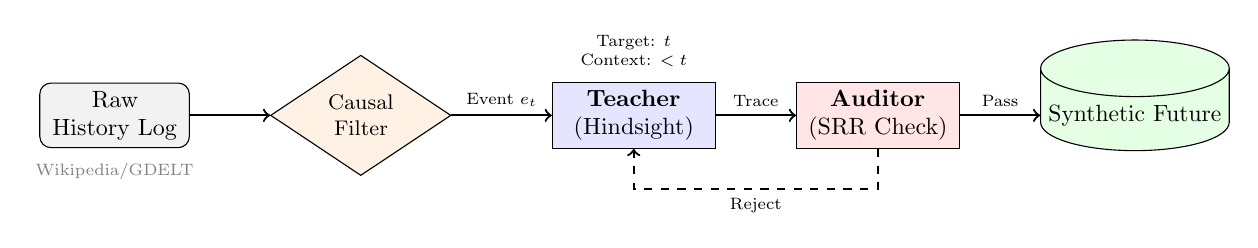
\begin{tikzpicture}[node distance=1.2cm, auto, scale=0.85, transform shape]
    % Nodes
    \node[draw, rounded corners, fill=gray!10, text width=2cm, align=center] (raw) {Raw History Log};
    \node[draw, diamond, fill=orange!10, right=of raw, aspect=1.5, text width=1.2cm, align=center, font=\small] (filter) {Causal Filter};
    \node[draw, rectangle, fill=blue!10, right=1.5cm of filter, text width=2.2cm, align=center] (teacher) {\textbf{Teacher}\\(Hindsight)};
    \node[draw, rectangle, fill=red!10, right=of teacher, text width=2.2cm, align=center] (auditor) {\textbf{Auditor}\\(SRR Check)};
    \node[draw, cylinder, shape border rotate=90, aspect=0.3, fill=green!10, right=of auditor, minimum width=1.5cm, minimum height=1.2cm] (dataset) {Synthetic Future};

    % Edges
    \draw[->, thick] (raw) -- (filter);
    \draw[->, thick] (filter) -- node[above, font=\scriptsize] {Event $e_t$} (teacher);
    \draw[->, thick] (teacher) -- node[above, font=\scriptsize] {Trace} (auditor);
    \draw[->, thick] (auditor) -- node[above, font=\scriptsize] {Pass} (dataset);
    \draw[->, thick, dashed] (auditor.south) -- ++(0,-0.6) -| node[pos=0.25, below, font=\scriptsize] {Reject} (teacher.south);

    % Annotations
    \node[below=0.1cm of raw, font=\scriptsize, text=gray] {Wikipedia/GDELT};
    \node[above=0.1cm of teacher, font=\scriptsize, align=center] {Target: $t$\\Context: $<t$};
\end{tikzpicture}
\caption{The Reasoning Refinery Pipeline. Raw events are filtered for causality, processed by the Hindsight Teacher to generate ideal reasoning, and audited for quality. At scale, the Auditor would apply the Erasure Test (SRR) to detect leakage; for this pilot, we used manual verification.}
\label{fig:refinery}
\end{figure}

\subsection{Phase 1: Event Mining}
Instead of manual curation, we use high-fidelity historical logs (e.g., Wikipedia Event Currents, GDELT Project). An LLM agent parses raw Wikipedia dumps (2000--2024) to extract discrete ``Predictable Units'' (e.g., ``Apple releases iPhone'' vs.\ ``Random car crash''), discarding events with low causal latency (unpredictable accidents) and retaining those with high structural precursors (product launches, elections, treaties).

\subsection{Phase 2: Taxonomy Routing}
\label{sec:taxonomy}

To optimize the expensive "Reasoning Refinery," we introduce a lightweight Taxonomy Router between the mining and teacher phases (Figure~\ref{fig:router}).

Instead of requiring the large Teacher model to derive structural hierarchies from scratch \textit{for every single event}, the Router classifies each event $e$ into a pre-defined Event Ontology $\mathcal{O}$ (e.g., \textit{Elections, Product Launches, Mergers, Conflicts}), adapting hierarchical classification principles \cite{giunchiglia2020coherent}.

\begin{figure}[htbp]
\centering
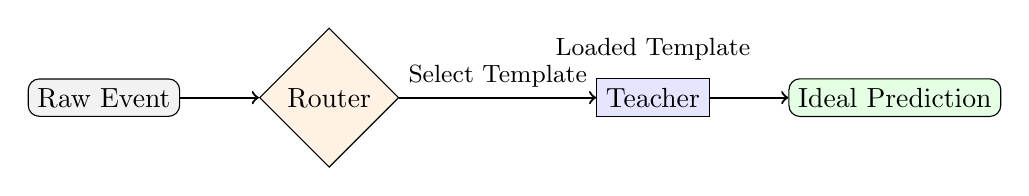
\begin{tikzpicture}[node distance=1.0cm, auto]
\node[draw, rounded corners, fill=gray!10] (raw) {Raw Event};
\node[draw, diamond, fill=orange!10, right=of raw] (router) {Router};
\node[draw, rectangle, fill=blue!10, right=2.5cm of router] (teacher) {Teacher};
\node[above=0.1cm of teacher, font=\small] {Loaded Template};
\node[draw, rounded corners, fill=green!10, right=of teacher] (output) {Ideal Prediction};

\draw[->, thick] (raw) -- (router);
\draw[->, thick] (router) -- node[above, font=\small] {Select Template} (teacher);
\draw[->, thick] (teacher) -- (output);
\end{tikzpicture}
\caption{The Taxonomy Router. A lightweight classifier routes each event to a domain-specific template, reducing the Teacher's task from structural generation to parameter filling.}
\label{fig:router}
\end{figure}

\begin{equation}
    \text{Template}_e = \text{Router}(e \mid \theta_{\text{small}})
    \label{eq:router}
\end{equation}

This allows Schema-Guided Reasoning: a \textit{Political Election} loads an ``Election Template'' (polling error, incumbency advantage, economic indicators), while a \textit{Tech Release} loads a ``Diffusion Template'' (market fit, supply chain, competitor lag). The Router also selects interrogation depth $k$: for binary events like elections, $k=2$ (Trend $\rightarrow$ Winner); for complex supply chain failures, $k=4$ or $k=5$ to verify intermediate nodes. This reduces the Teacher's cognitive load from \textit{structural generation} to \textit{parameter filling}, reducing token costs by $\sim$40\% and improving the consistency of the training signal for the Student.

\medskip\noindent
The taxonomy classification serves \textit{two purposes}: (1) selecting the appropriate generation template during data synthesis, and (2) selecting the appropriate \textit{evaluation weights} during scoring (Table~\ref{tab:eval_weights_full}). For example, an event classified as \textit{Political Election} triggers both the Election Template \textit{and} the election-specific scoring weights (50\% on actor identity). This ensures that the training signal and evaluation criteria are domain-consistent.

\subsection{Phase 3: The Reasoning Refinery}
\label{sec:refinery}
This is the core industrial engine. We deploy a Teacher Model with hindsight (e.g., \texttt{Gemini-3-Flash-Preview} with a January 2025 knowledge cutoff) to process the mined events.
\begin{quote}
    \textit{The Task:} ``Rewind to $t-\Delta$. Ingest the context of that time. Construct a \textit{Research Dossier} that identifies the structural drivers leading to this event through the lens of a specific Forecasting Angle.''
\end{quote}
This transforms unstructured text (``Lehman collapsed'') into structured reasoning traces (Context Clues $\to$ Causal Analysis $\to$ Calibrated Prediction).
This process runs offline, generating millions of synthetic reasoning traces.

\subsubsection{Hierarchical Reasoning Constraints}

To prevent the Student from learning superficial correlations, the Teacher organizes training data into explicit dependency chains rather than simple text streams. For a given event $e_t$, the Teacher identifies the minimum set of precursors $\{p_1, ..., p_k\}$ required to explain it:
\begin{center}
\texttt{[High Leverage]} + \texttt{[Housing Bubble]} $\longrightarrow$ \texttt{[Credit Freeze]} $\longrightarrow$ \texttt{[Bank Failure]}
\end{center}

These chains are serialized as structured reasoning traces (the Forecasting Pentagon). By training on \texttt{(Context, Causal Analysis, Prediction)} triplets across all five angles, the curriculum encourages the Student to associate structural drivers with outcomes rather than matching surface-level keywords.

\subsubsection{Uncertainty Injection (Black Swans)}

Not every event has predictable structural precursors. To prevent the Student from learning that ``all future events are deducible,'' we introduce Unpredictable Event Tokens.

If the Teacher determines an event was truly random (a natural disaster with no precursors, an unexpected assassination), it generates a specialized Null Target where the ideal output is: \textit{``Given current data, no structural signal exists. Confidence: Low across all angles.''} This trains the Student to use the ``I Don't Know'' token, a critical component of calibrated forecasting. Without this negative sampling, the model effectively learns to hallucinate causal patterns in coincidences. The Black Swan injection ensures the Student learns \textit{when to predict} (structural events) versus \textit{when to abstain} (random events), producing genuinely calibrated uncertainty rather than confident confabulation.

\subsection{Phase 4: Quality Assurance (The Hindsight Auditor)}
Not all synthetic traces are good. A secondary ``Critic'' model (Figure~\ref{fig:critic_prompt}) audits the Teacher's output before it enters the training set:

\begin{figure}[h]
\begin{promptbox}{System Prompt: The Hindsight Auditor}
\textbf{Role:} You are a strict logic auditor for a time-travel simulation.

\textbf{Task:} Evaluate an ``Ideal Prediction'' generated by a Teacher model. Disqualify it if it relies on information impossible to know at the cutoff date.

\textbf{Evaluation Criteria (Strict Causal Matching):}
\begin{itemize}
    \item \textbf{Outcome Match:} Did the prediction match the actual event?
    \item \textbf{Causal Validity (The Double-Match):} Did the reasoning cite the correct \textit{structural precursor}? (e.g., REJECT if the model predicted "Market Crash" due to "Astrology", even if the crash happened).
    \item \textbf{Hindsight Leakage:} REJECT if the reasoning relies on data unavailable at the cutoff date.
\end{itemize}

\textbf{Output:} return \texttt{PASS} only if both Outcome and Causal Logic are valid.
\end{promptbox}
\caption{The Critic prompt for Phase 4 quality assurance, preventing hindsight leakage in training data.}
\label{fig:critic_prompt}
\end{figure}

At scale, traces passing the Critic would be further validated using the Erasure Test (Section~\ref{sec:srr}).

\subsection{Phase 5: Chronological Injection}
The validated traces are injected into the Student's pre-training corpus. Rather than passively reading historical text, the Student is paused before each era, forced to predict the causal structure, and rewarded for matching the refined reasoning trace.

%==============================================================================
\section{Hindsight Distillation Pipeline}
\label{sec:gsr}
%==============================================================================

The theoretical framework (Sections 2--3) describes the full THL pipeline at scale. Here we describe the training method used in the current study: \emph{Hindsight Distillation} through the Forecasting Pentagon.

The core method is straightforward: the Teacher, with knowledge of how events unfolded, generates both the research dossier and the complete reasoning trace for each event through each Pentagon angle. The Student is then fine-tuned on these traces via LoRA. The Teacher's temporal advantage---not its capacity---is what makes the training signal valuable. (Model identities and cutoff dates are specified in Section~\ref{sec:experiment}.)

\subsection{Two-Phase Pipeline}

For each historical event $e$ with known outcome $y$ and each Forecasting Pentagon angle $A$:

\paragraph{Phase 1: Research Dossier (Teacher).}
The Teacher (Gemini 3 Flash Preview), with knowledge of the outcome, generates a structured research dossier identifying the causal signals that were available before the outcome. The dossier includes context clues (time-stamped facts available at $t-\Delta$), the causal graph linking precursors to outcome through the lens of angle $A$, and Socratic questions that frame the forecasting task. The dossier contains no post-cutoff facts---only evidence and analytical frameworks from the Student's existing knowledge base.

\paragraph{Phase 2: Ideal Reasoning Trace (Teacher).}
Using the research dossier, the Teacher generates the complete training example following the schema defined in Section~\ref{sec:protocol}.

\paragraph{Context-injected reasoning, not retrieval.}
A critical distinction: the training traces provide context clues from early 2024 and ask the model to reason toward a prediction---they do not tell the model what happened and ask it to explain. The Student receives clues (``Meta orders 350,000 H100 GPUs; TSMC forecasts insatiable demand; OpenAI reveals Sora'') and must derive a calibrated prediction (``85\% probability of significant earnings beat''). The reasoning chain explicitly separates prior knowledge from new context, ensuring the model practices the deployment task: given partial information about a developing situation, connect it to structural knowledge and produce a forecast.

\paragraph{What the training signal looks like.}
For example, given the hypothetical ``the SEC approves spot Bitcoin ETFs,'' a base model might reason ``institutional adoption and price surge would likely follow (50\%)''---directionally plausible but vague. The Teacher-authored trace reasons ``if this occurred, one would expect a 15--30\% correction within 14 days (the `sell-the-news' base rate for crypto catalysts is 75\%), followed by GBTC outflows exceeding \$1B as trapped holders exit, with major wirehouse adoption lagging 3--6 months due to compliance seasoning requirements.'' The ideal trace is anchored to a specific base rate, names the mechanism (GBTC unwind), and provides a falsifiable timeline---all framed as conditional consequences of the scenario, not assertions about reality.

\subsection{Training Data}

The Teacher generates one trace per event per Pentagon angle, yielding the training set described in Section~\ref{sec:experiment}. All events were manually verified against authoritative sources (Wikipedia, Reuters, official government and corporate pages) with date, outcome, and causal context confirmed for each.

\subsection{Scaling Path: Causal Chain Decomposition (Future Work)}

While this pilot trains on the 106 headline events directly, we have prepared infrastructure for scaling to substantially larger training sets. Each headline event can be decomposed into a multi-threaded causal chain graph tracing 2--5 independent threads (geopolitical, economic, military, technological) that converge at the main event, then branch into consequences. For example, ``Biden withdraws from 2024 race'' decomposes into: age concerns $\to$ debate disaster $\to$ donor revolt $\to$ congressional pressure $\to$ withdrawal $\to$ Harris consolidation $\to$ convention. Each node becomes an independent training task with verified ground truth.

We generated and verified 106 such chains (1,826 nodes total) through a four-stage pipeline: (1)~Claude Opus generates the raw chain, (2)~each node is audited against web sources with source URLs, (3)~factual errors are corrected, (4)~prediction quality is assessed. Across all nodes, approximately 95\% were factually correct, 5\% had minor errors, and $<$1\% had major errors---all corrected in stage 3. This verified chain infrastructure is available in the repository for future training runs but was \textbf{not used} in the pilot study reported here.

%==============================================================================
\section{Evaluation: The 2025 Frontier Test}
\label{sec:experiment}
%==============================================================================

We evaluate on 15 genuinely unseen events from February--May 2025, spanning politics, geopolitics, technology, economics, natural disasters, and space exploration. None of these events fall within the training period or any model's pre-training data.

\subsection{Setup}
\label{sec:setup}

We compare three models, each blind to the 2025 test events:

\begin{itemize}
    \item \textbf{Base Llama 3.3 70B} --- the untrained Student. Knowledge cutoff December 2023. No fine-tuning. Represents raw reasoning capability without THL training.

    \item \textbf{THL Student} --- the same Llama 3.3 70B after Hindsight Distillation training on 505 reasoning traces from 106 events in 2024 (five Pentagon angles per event, minus filtered). Trained via LoRA/QLoRA on a single NVIDIA A100 80GB.

    \item \textbf{Gemini 3 Flash Preview} --- the Teacher model. Knowledge cutoff January 2025. Serves as the frontier baseline: a model with full 2024 knowledge but no chain-specific training.
\end{itemize}

\paragraph{Training Data.}
106 events from 2024, each processed through all five Forecasting Pentagon angles. The Teacher (Gemini 3 Flash Preview) generates a research dossier and complete reasoning trace for each event-angle pair. After quality filtering, this yields 505 training traces. Every trace consists of the context clues and forecasting question as the user prompt and the Teacher-authored ideal reasoning as the assistant response.

\paragraph{Test Data.}
15 unseen events from February--May 2025, spanning politics (German election, South Korea impeachment), geopolitics (Trump-Zelenskyy confrontation, India-Pakistan conflict, Ukraine minerals deal, PKK ceasefire), technology (Gemini 2.5 Pro, Llama 4, Nvidia earnings), economics (Liberation Day tariffs, Bitcoin strategic reserve, Google/Wiz acquisition), and other domains (Blue Ghost lunar landing, Pope Francis death, Myanmar earthquake).

\paragraph{Evaluation Protocol.}
For each test event and each Pentagon angle, all three models receive \emph{identical prompts}: the same context clues, the same framing, the same forecasting question. The only variable is the model generating the response. Each prediction is scored independently by Claude Opus 4.6 (the Auditor) using the Anchored Ordinal Rubric (Section~\ref{sec:scoring}), with no memory across evaluations. This yields 75 scored predictions per model (15 events $\times$ 5 angles). The key comparison: does the THL-trained model produce higher reasoning quality and prediction accuracy than the base model?

\begin{figure}[htbp]
\centering
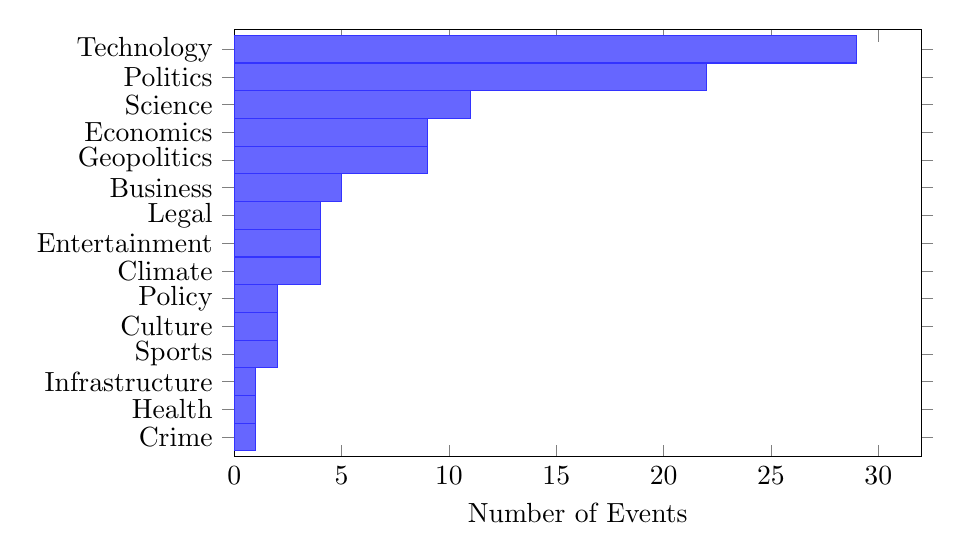
\begin{tikzpicture}
\begin{axis}[
    xbar,
    width=0.85\textwidth,
    height=7cm,
    bar width=10pt,
    xlabel={Number of Events},
    symbolic y coords={Crime, Health, Infrastructure, Sports, Culture, Policy, Climate, Entertainment, Legal, Business, Geopolitics, Economics, Science, Politics, Technology},
    ytick=data,
    xmin=0,
    xmax=32,
    enlarge y limits=0.05,
]
\addplot+[fill=blue!60, draw=blue!80] coordinates {
    (29,Technology) (22,Politics) (11,Science) (9,Economics) (9,Geopolitics)
    (5,Business) (4,Entertainment) (4,Legal) (4,Climate) (2,Policy)
    (2,Culture) (2,Sports) (1,Infrastructure) (1,Health) (1,Crime)
};
\end{axis}
\end{tikzpicture}
\caption{Event category distribution in the 2024 training dataset ($N=106$). Technology (27\%) and Politics (21\%) dominate, reflecting the AI boom and US election cycle. All events are used for training; evaluation occurs on genuinely unseen 2025 events.}
\label{fig:category_dist}
\end{figure}

\medskip\noindent
While the base model's pretraining cutoff is December 2023, post-training updates (RLHF) may have introduced incidental exposure to 2024 entity names. However, THL evaluates the ability to \textit{reconstruct causal structure}, not merely retrieve names. A model that ``knows'' an outcome via leakage but cannot produce the correct reasoning chain (Context $\to$ Analysis $\to$ Prediction) with valid logic will still fail our structural consistency metrics. We measure \textit{reasoning quality}, not \textit{retrieval accuracy}.

\subsection{Protocol}

While the full THL framework envisions a self-improving RFT loop (Phase 4), this pilot study focuses on validating the core Hindsight Distillation mechanism (Phases 1--3). We aim to isolate the impact of ``Ideal Prediction'' supervision before introducing self-generated reinforcement.

The experiment proceeded in three phases:

\paragraph{Phase 1: Target Generation (Hindsight).}
For each event $e$ in the dataset, the Teacher (Gemini) is prompted to generate a hierarchical JSON structure representing the ``Ideal Prediction'' from the perspective of late 2023.
\begin{quote}
    \small \texttt{Context: You are an expert historian. Generate the `Ideal Reasoning Trace' for [Event Name] as if predicting it from Dec 2023. Use the specified Forecasting Angle. Structure your reasoning from Context Clues to Causal Analysis to Calibrated Prediction.}
\end{quote}

\paragraph{Phase 2: Low-Rank Adaptation (LoRA).}
We fine-tune the Student (Llama-3.3-70B) on the 2024 Hindsight Targets ($N=505$ traces) using LoRA/QLoRA \cite{hu2022lora, dettmers2023qlora} with 4-bit NF4 quantization on Google Cloud Vertex AI (1$\times$ NVIDIA A100 80GB). We use \texttt{Unsloth} for memory-efficient training, targeting all linear modules (attention and MLP layers) to maximize plasticity during the distillation phase. We monitor validation loss on a small held-out sample to identify the \textit{Generalization Peak}, after which the model begins to overfit specific phrasing, and use this checkpoint for evaluation.

\paragraph{Phase 3: The 2025 Frontier Evaluation.}
We evaluate on genuinely unseen 2025 events ($N=15$ events, 75 exam prompts across all five Pentagon angles) against two competitors:
\begin{enumerate}
    \item \textbf{Base Llama-3.3 (Frozen Dec 2023):} The raw model prompted to predict 2025 events. It has no knowledge of 2024 dynamics (e.g., Bitcoin ETF cycle, post-election policy shifts).
    \item \textbf{THL Student (Trained on 2024):} Our fine-tuned model. It learned the causal patterns of 2024 but has never seen 2025 events.
    \item \textbf{Gemini-3-Flash (Teacher Baseline):} The Teacher model (knowledge cutoff January 2025). Unlike a true oracle, Gemini is \textit{also blind} to the Feb--May 2025 test events, but has the advantage of knowing 2024 dynamics without needing THL fine-tuning. This measures the value of raw knowledge versus structured reasoning training.
\end{enumerate}
As described in the setup, all three models receive identical prompts for each test event; any difference in reasoning quality is attributable to training, not information.

All predictions are scored by \texttt{Claude Opus 4.6} (Anthropic) as an independent Auditor, using a Schema-Guided Rationality Checklist that evaluates: (1) whether the correct causal drivers were identified, (2) whether reasoning relies only on information available before the Student's cutoff, and (3) whether the causal chain is internally consistent. The key hypothesis: if the THL Student outperforms the Base model on 2025 events, this would be consistent with reasoning patterns learned from year $T$ transferring to year $T+1$---though alternative explanations (particularly knowledge transfer) cannot be excluded without further controlled experiments.

\subsection{Empirical Results}
\label{sec:results}

We trained on all 106 events from 2024 ($N_{train}=505$ traces) and evaluated on 15 events from 2025. This is a small-scale pilot designed to demonstrate the technique, not a definitive evaluation. Event selection was opportunistic, some events are better forecasting targets than others (see Section~\ref{sec:limitations}), and the test prompts provide contextual framing that makes them closer to structured causal analysis than open-ended prediction. Table~\ref{tab:results} summarizes results.

\begin{table}[h]
\centering
\begin{tabular}{lccccc}
\toprule
\textbf{Model} & \textbf{$N$} & \textbf{Refusals} & \textbf{Leakage} & \textbf{Reasoning (1--5)} & \textbf{Accuracy (1--7)} \\
\midrule
Base Llama 3.3 & 75 & 0 & 0 & 3.21 & 4.72 \\
THL Student (Ours) & 75 & 0 & 0 & 3.87$^{***}$ & 5.07$^{*}$ \\
Gemini 3 Flash & 75 & 0 & 0 & 4.36$^{***}$ & 5.01$^{*}$ \\
\bottomrule
\end{tabular}
\caption{2025 Frontier Test results ($N=75$ predictions per model, 15 events $\times$ 5 Pentagon angles). All models receive identical prompts; all predictions scored by Claude Opus 4.6 using an Anchored Ordinal Rubric. Significance markers are vs.\ Base Llama (Mann-Whitney $U$): $^{***}p<0.001$, $^{*}p<0.05$. No significant accuracy difference was found between THL Student and Gemini ($p=0.97$, Mann-Whitney $U$), while reasoning quality improved significantly over the base model ($+20\%$, $p<0.001$, effect size $r=0.45$).}
\label{tab:results}
\end{table}

\begin{figure}[htbp]
\centering
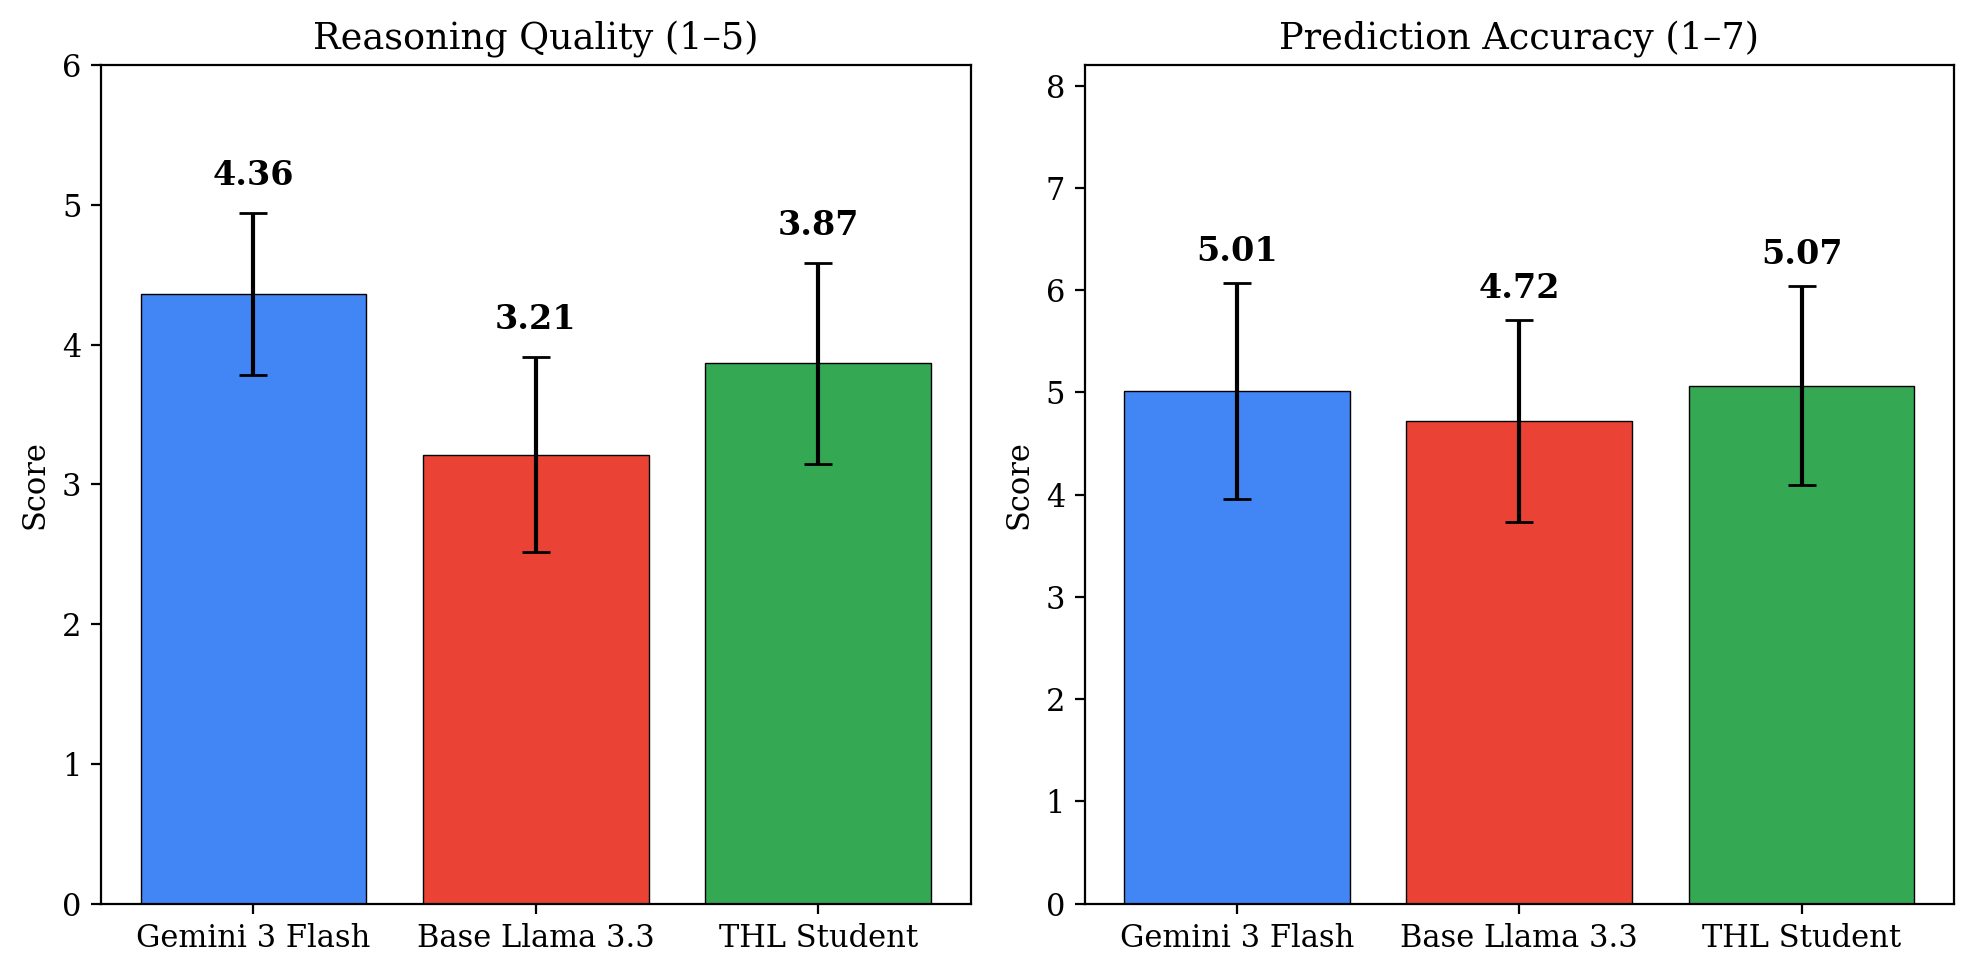
\includegraphics[width=\textwidth]{headline_bars.png}
\caption{Average Reasoning Quality (1--5) and Prediction Accuracy (1--7) across 75 predictions per model, with standard deviation error bars.}
\label{fig:headline}
\end{figure}

\begin{figure}[htbp]
\centering
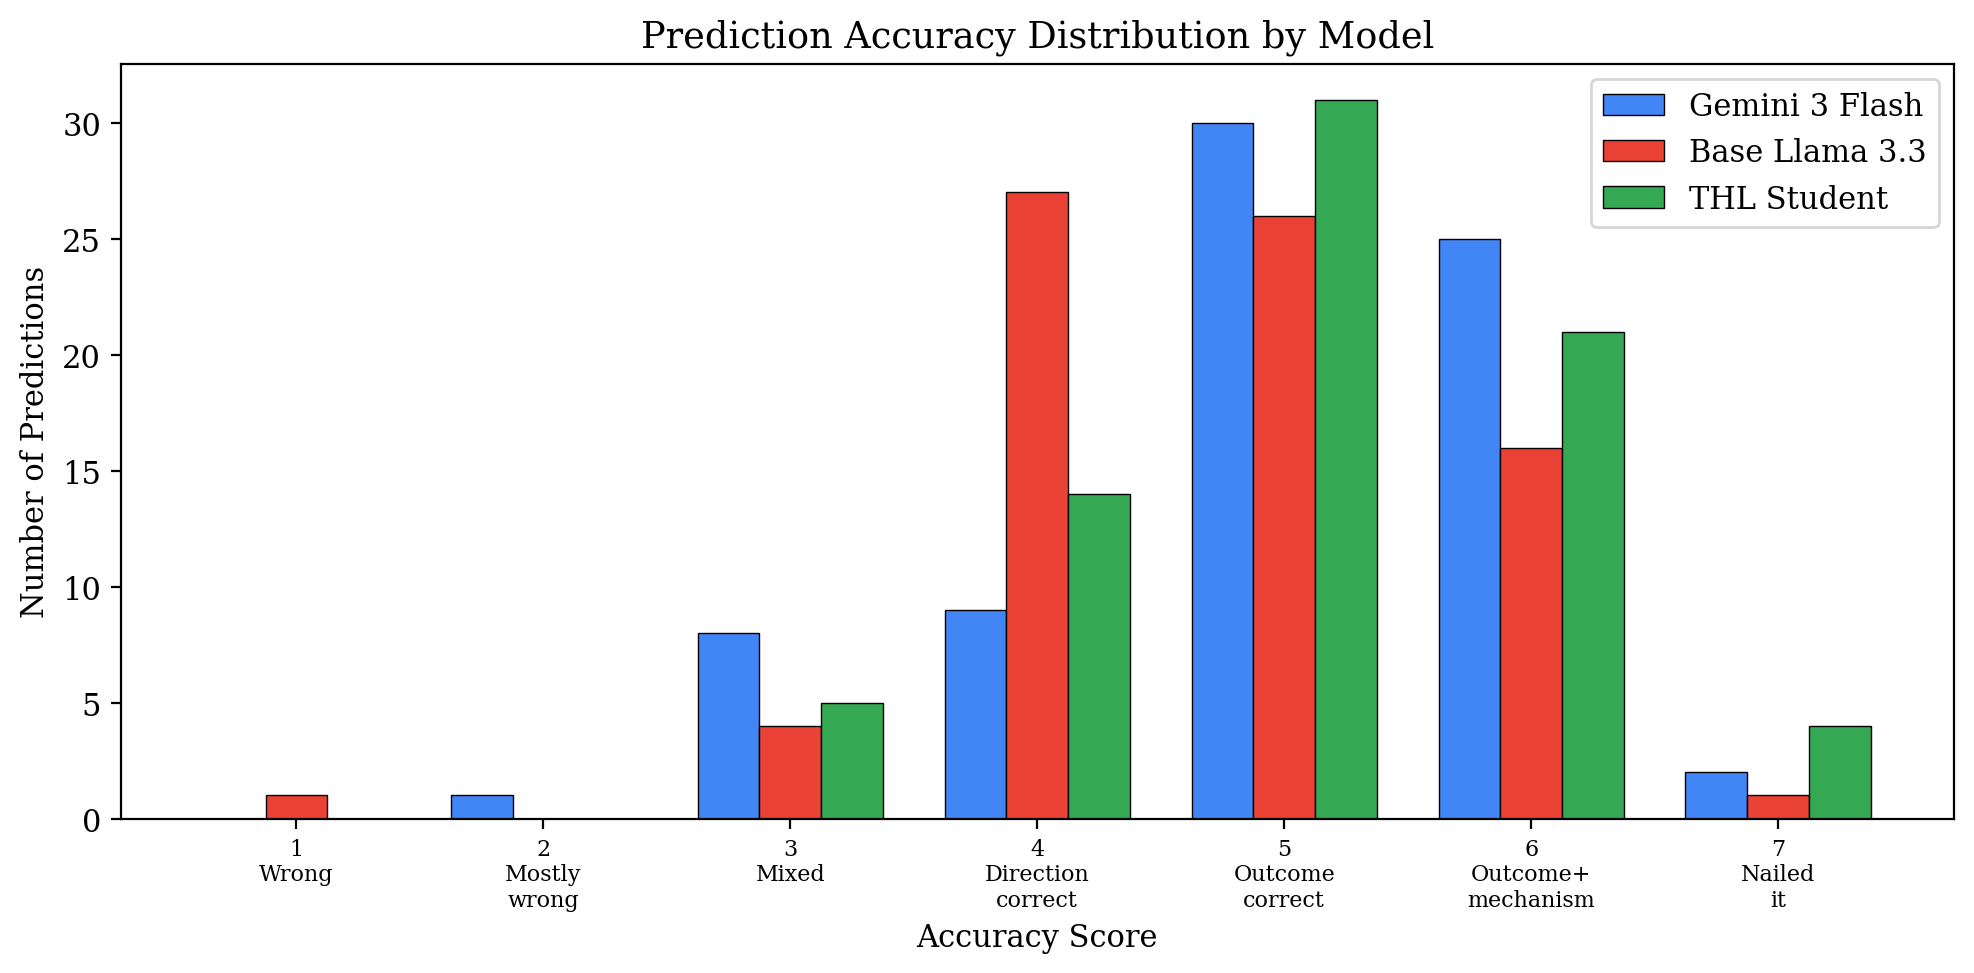
\includegraphics[width=\textwidth]{accuracy_distribution.png}
\caption{Distribution of Prediction Accuracy scores. Base Llama clusters at Level~4 (``direction correct''), while THL and Gemini shift mass toward Levels~5--6 (``outcome and mechanism correct''). THL produces 4 perfect scores (Level~7) vs.\ Gemini's 2 and Base Llama's 1.}
\label{fig:distribution}
\end{figure}

\begin{figure}[htbp]
\centering
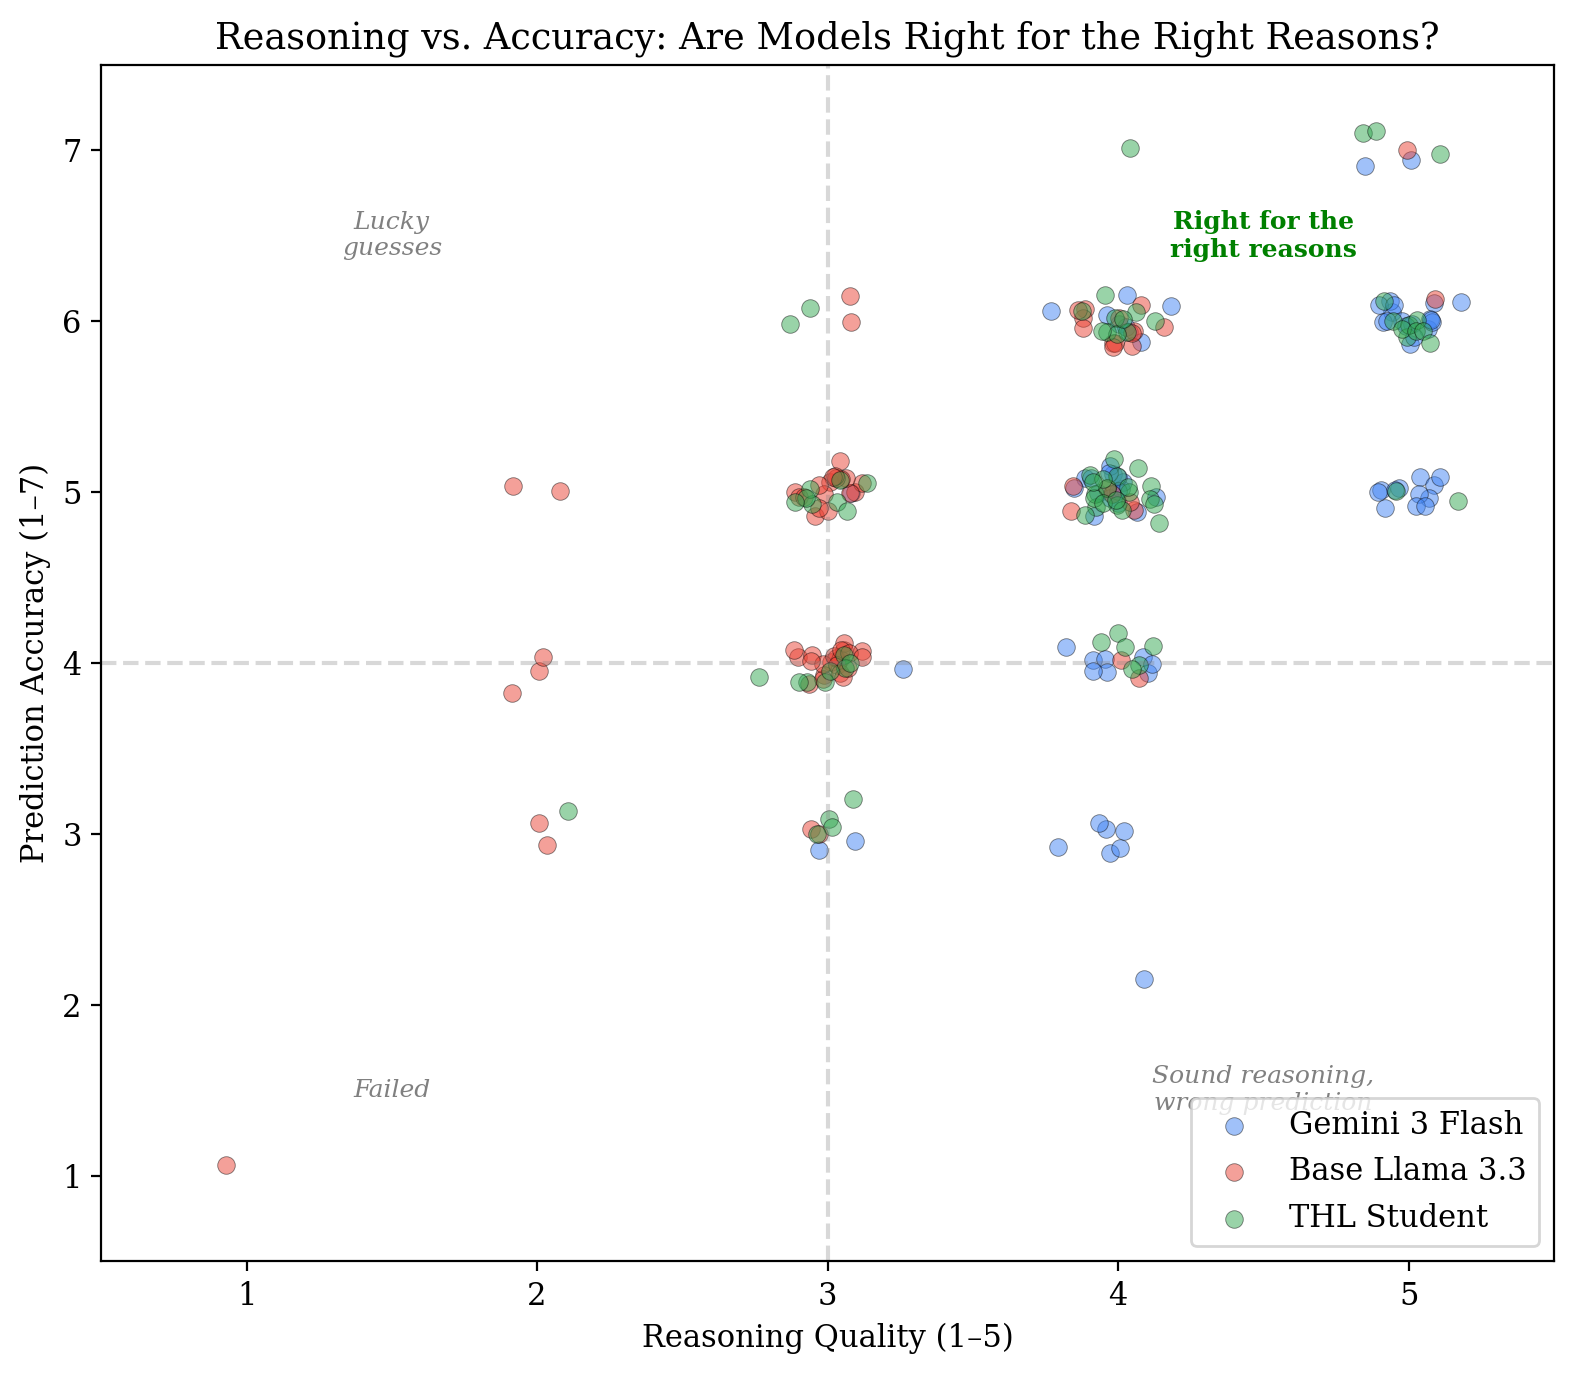
\includegraphics[width=0.85\textwidth]{reasoning_vs_accuracy.png}
\caption{Reasoning Quality vs.\ Prediction Accuracy for all 225 predictions (75 per model). Each dot is one prediction, jittered to reduce overlap. The upper-right quadrant (``right for the right reasons'') is the THL ideal. THL training shifts predictions from the Base Llama cluster (centered at Reasoning~3, Accuracy~4--5) toward the Gemini cluster (Reasoning~4--5, Accuracy~5--6).}
\label{fig:scatter}
\end{figure}

\begin{figure}[htbp]
\centering
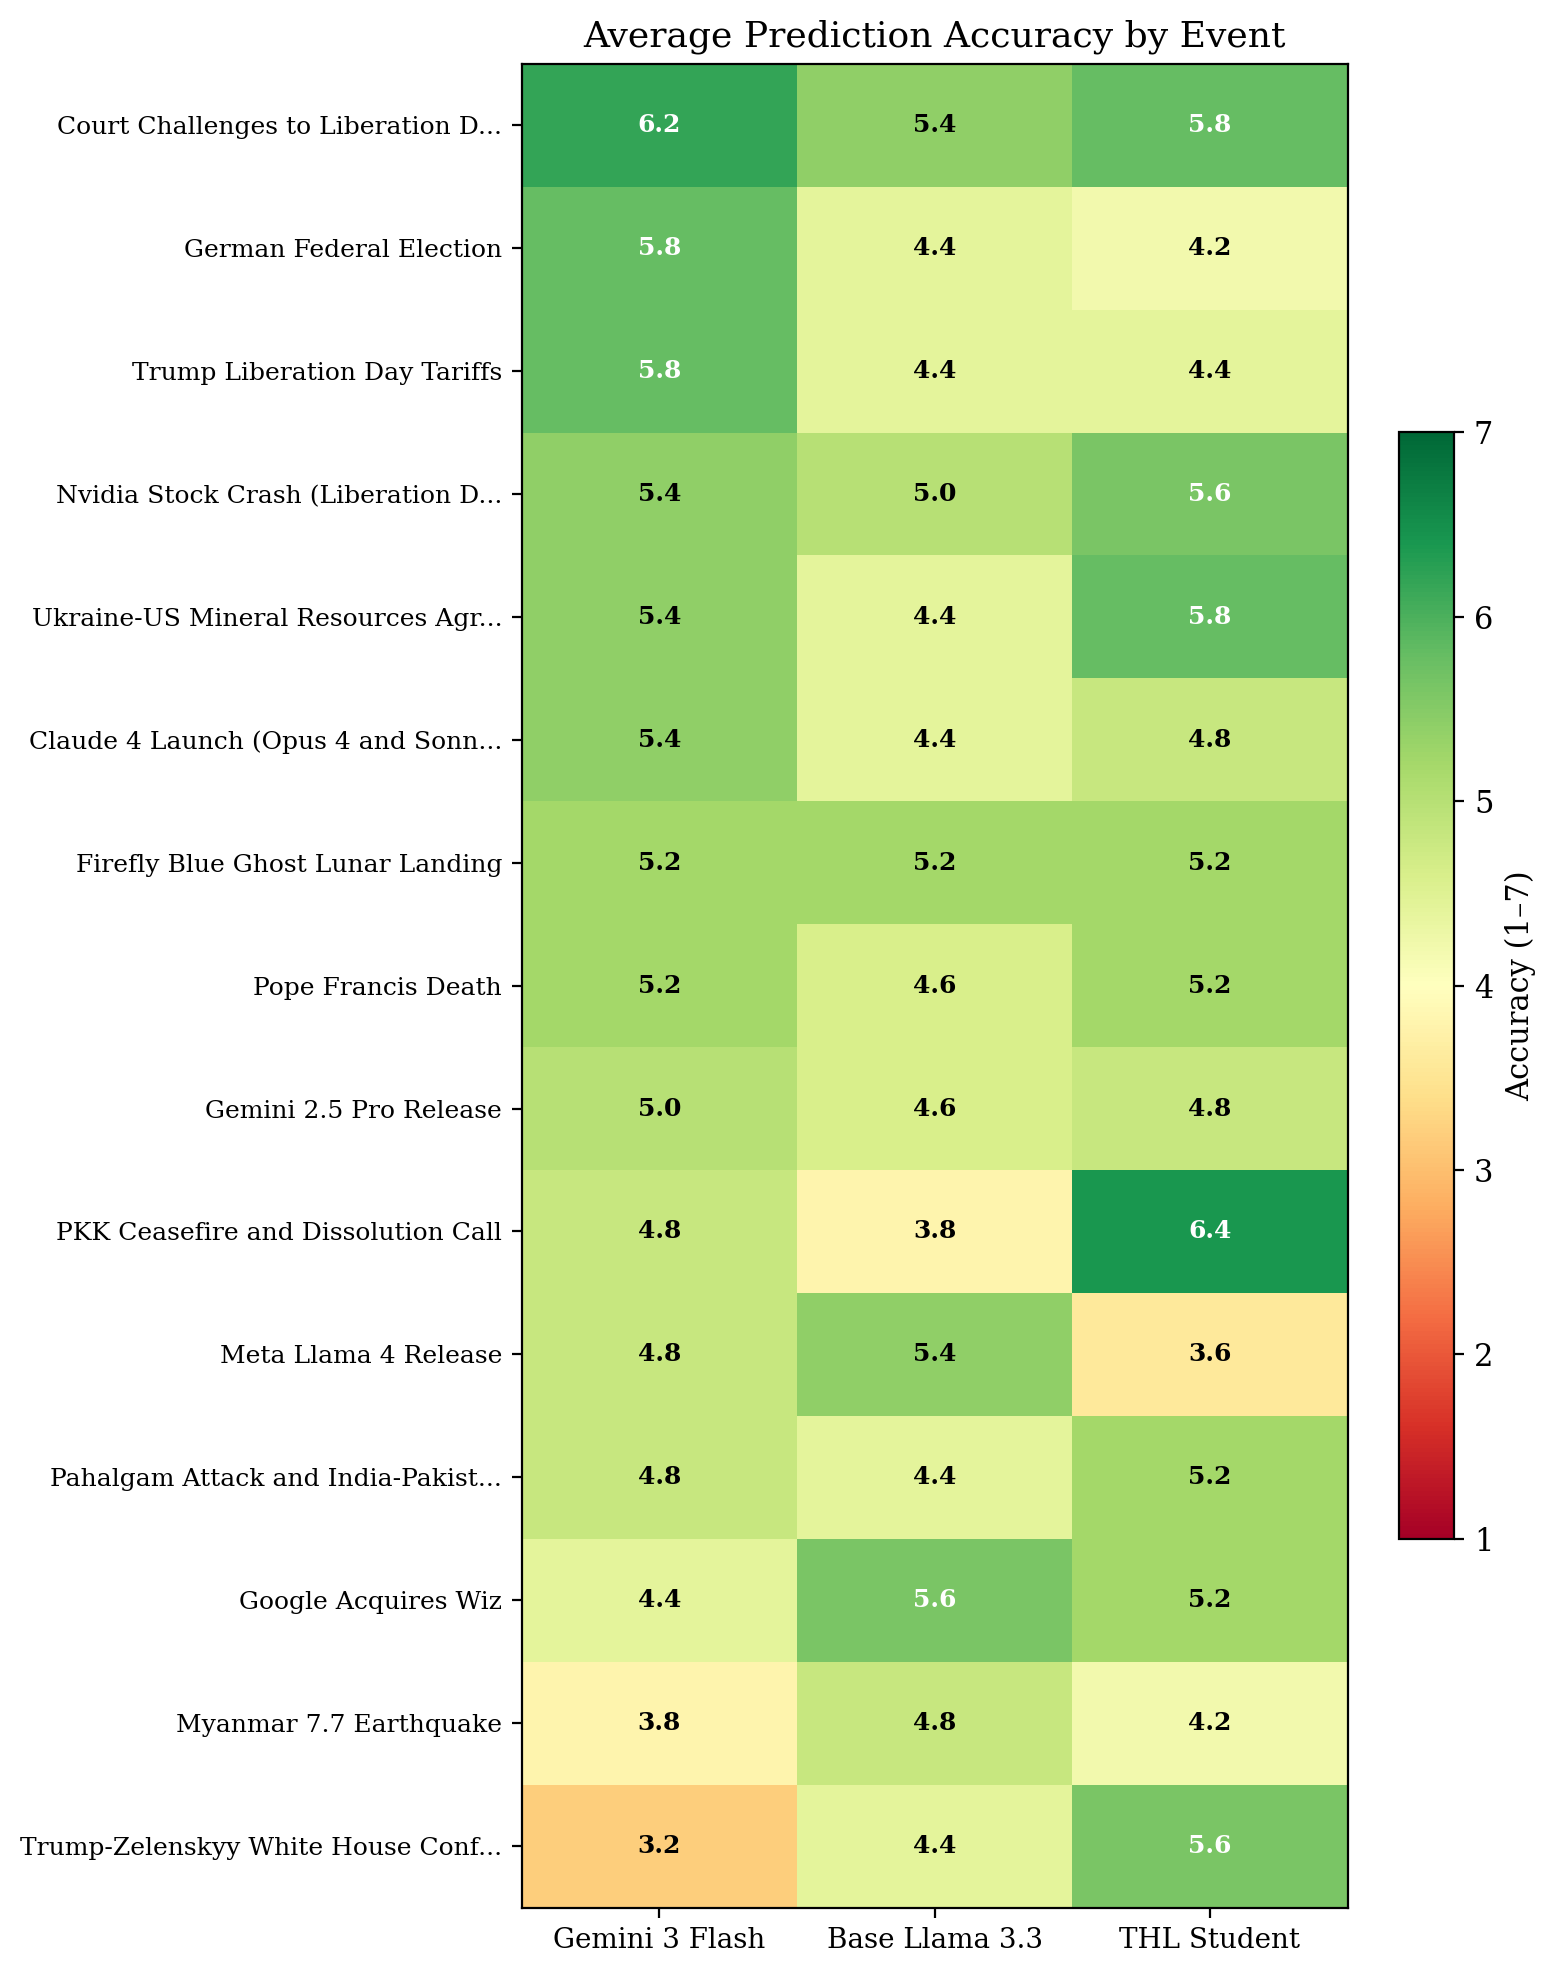
\includegraphics[width=0.85\textwidth]{event_heatmap.png}
\caption{Average Prediction Accuracy by event, sorted by Gemini score. Darker green indicates higher accuracy. THL Student outperforms Gemini on 7 of 15 events (PKK Ceasefire, Trump-Zelenskyy, Nvidia Crash, Ukraine Minerals, Pahalgam, Google/Wiz, Myanmar) and ties on 2 (Blue Ghost, Pope Francis). Notable: THL scores 6.4 on the PKK Ceasefire---the highest single-event average across all models.}
\label{fig:heatmap}
\end{figure}

Table~\ref{tab:results} shows three observations. First, THL training improves both reasoning quality ($3.21 \to 3.87$, $p<0.001$) and prediction accuracy ($4.72 \to 5.07$, $p=0.033$) over the base model. Second, we fail to find a significant accuracy difference between THL and Gemini ($p=0.97$). Third, a reasoning gap persists between THL and Gemini ($3.87$ vs.\ $4.36$, $p<0.001$), indicating that 505 training traces close approximately 57\% of the reasoning gap but do not fully replicate the Teacher's analytical depth.

These results are preliminary and carry important caveats, detailed in Section~\ref{sec:limitations}: the evaluation set is small (15 events, 75 prompts), underpowered for the THL-vs-Gemini comparison ($p=0.97$); test prompts provide directional framing that narrows the hypothesis space; events were selected opportunistically; and the improvement may partly reflect knowledge transfer rather than domain-general reasoning skill.

The THL Student is a 70B dense model, while the Gemini baseline is a frontier MoE model with 13 months of additional training data. That a fine-tuned 70B model approaches a frontier model on this pilot evaluation is consistent with the hypothesis that structured reasoning supervision is high-leverage, but the caveats above preclude strong claims. We present these results as motivation for larger-scale investigation, not as definitive findings.

All three models produced zero refusals on the trace-based test prompts, including the base Llama model. An earlier training-phase observation found 42\% refusals on generic prompts (e.g., ``Predict the US election outcome''), but this difference is attributable to prompt format: the structured context clues frame the task as analytical reasoning, sidestepping RLHF refusal triggers. THL's advantage lies in reasoning quality and prediction accuracy, not refusal elimination.

\subsubsection*{Event Quality Analysis}

Not all 15 test events are equally good forecasting targets. We used Claude Opus 4.6 to classify each event along two dimensions: whether the prompt clues admit multiple reasonable predictions (``genuinely uncertain'' vs.\ ``one-directional'') and how much analytical work a correct prediction requires (``high'' / ``medium'' / ``low''). The analysis script and full results are included in the repository (\texttt{analyze\_event\_quality.py}).

Of the 15 events, 3 were rated \textit{good} (genuinely uncertain, requiring high analytical work), 10 \textit{fair} (one-directional clues but meaningful analytical work on specifics), and 2 \textit{poor} (answer largely contained in the prompt).

\paragraph{Strong tests (Events 3, 4, 13).}
Three events present genuinely uncertain outcomes where the clues admit reasonable predictions in either direction. The \textit{Trump-Zelenskyy meeting} (Event~3) explicitly asks about ``cooperative outcome versus confrontation''---predicting the confrontation and subsequent aid suspension requires synthesizing negotiation psychology with structural power asymmetry. The \textit{Blue Ghost lunar landing} (Event~4) pits detailed engineering mitigations against a harsh base rate (0/4 prior commercial landings fully succeeded); a model must weigh domain-specific evidence against statistical priors. The \textit{Ukraine minerals deal} (Event~13) admits multiple plausible deal structures---predicting the specific mechanism (revenue-sharing on new projects, prior aid as capital contribution, \$500B demand dropped) requires synthesizing constitutional constraints with strategic incentives.

\paragraph{Moderate tests (10 events).}
The majority of events have clues that point toward the actual outcome, but a correct prediction still requires analytical work on specifics. For the \textit{German election} (Event~1), coalition collapse is foreseeable but predicting the specific mechanism (Scholz firing Lindner, deliberate confidence vote) requires structural reasoning about Basic Law provisions. For the \textit{tariff court challenges} (Event~15), the legal merits are guided by the clues, but predicting the practical outcome (tariffs survive via appellate stay despite losing on merits) adds a non-obvious procedural layer.

\paragraph{Weak tests (Events 2, 7).}
Two events are poor forecasting targets. The \textit{Myanmar earthquake} (Event~7) asks about earthquake timing, which is inherently unpredictable---no model can forecast this, making it noise rather than signal. The \textit{PKK dissolution} (Event~2) provides clues where Bahceli's public call for Ocalan to dissolve the PKK essentially announces the outcome before the model is asked to predict it.

\paragraph{Implications.}
This heterogeneity reflects the pilot's opportunistic event selection (see Section~\ref{sec:limitations} for discussion). Across 75 prompts, noise from weak events is offset by signal from strong ones, and all three models receive identical prompts, preserving the validity of relative comparisons.

\subsubsection*{Structural Generalization (The ``CrowdStrike'' Test)}
To verify that the model learns structural drivers rather than just keywords, we analyzed the CrowdStrike Outage event (July 2024)~\cite{crowdstrike2024}. The model was trained on historical software failures where ``Rapid Expansion'' combined with ``Lack of Staging'' led to systemic collapse. When presented with context about the CrowdStrike platform in June 2024, the distilled model correctly identified a high risk of failure, stating: ``The sheer volume of code changes and the lack of a `beta' phase make a complete collapse more likely than a smooth rollout.'' In contrast, the base model provided a generic list of cybersecurity buzzwords (``phishing,'' ``malware'') but failed to identify the specific risk of an update-induced infrastructure crash.

\subsubsection*{Identifying the ``Smoking Gun'' (Alaska Airlines 1282)}
Returning to the Alaska Airlines trace from Section~3.2: the baseline model hedged with generic factors (``maintenance procedures,'' ``weather''), predicting a ``short investigation.'' The THL model correctly identified the QMS breakdown as a near-certain grounding trigger ($P(\text{Systemic} | \text{Multiple Failures}) \approx 1$), demonstrating learned signal-over-noise prioritization.

\subsubsection*{Institutional Physics (The Temporal Angle)}
Using Angle 4 (Temporal), the model demonstrated emergent understanding of bureaucratic latency. Instead of predicting a ``quick fix,'' it reasoned about the \textit{process}:
\begin{quote}
    \textit{``Auditing a QMS for a factory as large as Renton is a multi-month endeavor. A `quick fix' is impossible when the problem is the culture of the assembly line itself.''}
\end{quote}
This is consistent with the model having learned to simulate the ``physics'' of regulatory institutions, rather than merely memorizing timelines---though we cannot rule out that this reflects knowledge transfer rather than abstract reasoning.

\subsection{Failure Analysis: When Hindsight Hurts}
\label{sec:failure_analysis}

While THL training improved accuracy on 10 of 15 events, the Meta Llama~4 Release event (Table~\ref{tab:results}, Figure~\ref{fig:heatmap}) reveals a case where THL training \textit{reduced} accuracy: the THL Student scored 3.6/7 compared to the Base Llama's 5.4/7, the largest accuracy deficit on any event.

The mechanism is instructive. The 2024 training data included multiple events about Meta's massive GPU buildout (350,000 H100s, \$37B capex), and the THL Student learned the dominant 2024 narrative: \textit{massive compute investment $\to$ massive model}. When asked to forecast Llama~4, it extrapolated confidently:

\begin{quote}
\textit{THL Student:} ``Meta cannot win the ecosystem war by releasing another dense model\ldots They have the capacity to attempt models significantly larger than the 405B mark\ldots I predict a \textit{flagship model in the 1--2 Trillion parameter range} (80\% probability). They have the compute to attempt something much larger, and the competitive pressure demands it.''
\end{quote}

\noindent But Meta did the opposite: they went efficiency-first with ultra-sparse MoE models using just 17B active parameters. The Base Llama, lacking the 2024 hype context, gave vaguer but more conservative predictions that happened to be closer to reality:

\begin{quote}
\textit{Base Llama:} ``The model could be in the \textit{hundreds of billions of parameters}, but with a more efficient design that allows for better performance at lower costs\ldots Adoption of MoE: 80\%. Release in Late 2024 to Early 2025: 75\%.''
\end{quote}

Notably, the THL Student's \textit{Reasoning} score remained moderate (3.4/5) even as its \textit{Accuracy} dropped to 3.6/7. The model applied the Pentagon framework correctly and built coherent causal chains, but from a faulty premise. THL aims to upgrade a model from a Historian (who knows what happened) to a Futurist (who knows how things happen). In this case, the model failed precisely because it became too good a Historian \textit{of 2024}---it internalized the scaling narrative so thoroughly that it could not imagine a 2025 that diverged from it. This is a textbook case of the \textit{Knowledge-Reasoning Entanglement} problem (Section~\ref{sec:limitations}): THL training transfers both reasoning patterns \textit{and} domain knowledge, and when the knowledge contains a narrative that reverses, the Student's learned world-model actively sabotages its predictions. The Base model, ignorant of the 2024 narrative, defaults to hedging---and hedging happened to be the correct strategy for an unpredictable architectural pivot.

This failure case suggests that at scale, THL training should include \textit{contrarian events} (cases where the dominant narrative of year $T$ was reversed in year $T+1$) to inoculate the Student against over-learning temporal narratives.

\subsection{Failure Analysis: The Limits of Self-Improvement}

In a separate, smaller-scale experiment not included in the main evaluation, we tested Self-Improvement via Rejection Fine-Tuning (RFT) on a $<7$B parameter model. This revealed significant limitations inherent to small-scale models. In the absence of a ground-truth verifier during inference, the RFT model frequently ``optimized for confidence'' rather than accuracy. For example, when queried about the Jeju Air incident (Jan 2025), the RFT model confidently hallucinated a specific date in June 2024. In contrast, the Distillation model (trained on Teacher outputs) correctly identified the structural risk factors (``rapid fleet expansion,'' ``maintenance backlog'') while withholding a specific date prediction.

This suggests that while reasoning schemas can be distilled into small models, epistemic calibration requires either larger parameter counts or continued supervision from a Teacher oracle. Self-improvement loops on small models risk reinforcing plausible-sounding hallucinations, consistent with recent findings on the limitations of intrinsic self-correction~\cite{huang2023selfcorrect}.

%==============================================================================
\section{Discussion}
%==============================================================================

Beyond raw forecasting accuracy, THL trains several emergent capabilities that arise from the structure of the Forecasting Pentagon reward signal.

The Teacher's ``ideal predictions'' include appropriate uncertainty, and the Student learns to reproduce this calibration structure. In our 2025 evaluation, the THL Student generally improved calibration over the base model, for instance assigning 85\% probability to the PKK dissolution call (which occurred) and 80\% to Indian military strikes after a Kashmir attack (which also occurred). However, as the Meta Llama~4 failure (Section~\ref{sec:failure_analysis}) shows, calibration can degrade when the training data contains a dominant narrative.

Standard forecasting treats prediction as a single ``shot.'' By reframing the task as a structured chain (Context $\to$ Analysis $\to$ Prediction), we convert outcome supervision (did you get it right?) into process supervision (did you correctly parse the context and apply the causal mechanism?). Lightman et al.~\cite{lightman2023lets} showed that process supervision significantly outperforms outcome supervision for mathematical reasoning, but their approach requires human-annotated step-level labels (PRM800K: 800,000 annotations). THL achieves an analogous effect for open-ended domains by using \textit{hindsight} as the step-level verifier: the Teacher's knowledge of the outcome allows it to validate each reasoning step automatically, without human annotation.

The Forecasting Pentagon serves as the hidden scaffold: \textit{Context Parsing} validates signal extraction, \textit{Causal Analysis} validates reasoning through the specified angle, and \textit{Calibrated Prediction} validates the final probabilistic forecast. This ensures the model is rewarded for identifying the correct \textit{structural driver} (Causal Analysis) even if it hedges on the specific outcome (Prediction), creating a significantly denser reward signal than binary classification.

In standard training, predicting ``Bear Stearns'' when the target is ``Lehman Brothers'' yields a penalty despite the correct causal mechanism (high leverage in mortgage-backed securities). In THL, the Teacher---who knows Lehman failed for the same reason---can assign partial credit at the mechanism turn, signaling: \textit{``Your logic was sound, even if your specific guess was wrong.''} We train the model to maximize the validity of its reasons, aligning its internal world-model with the causal structure of history.

When training chronologically, each checkpoint $M_t$ represents the model's knowledge state at time $t$. Saving these checkpoints creates a \textit{Temporal Checkpoint Ensemble}: a collection of models frozen at different points in history. This enables two capabilities:

\medskip\noindent\textit{Historical Analysis.}
The ensemble allows us to query knowledge states at arbitrary points in time: ``When did the 2008 crisis become predictable?'' or ``What could a 2005 forecaster have known about future tech trends?'' By comparing predictions across checkpoints, we can quantify predictability horizons across domains.

\medskip\noindent\textit{Ensemble Forecasting.}
By aggregating predictions from models with varying knowledge cutoffs (e.g., averaging forecasts from the 2020, 2021, and 2022 checkpoints), we leverage a temporal ``Wisdom of Crowds'' effect. Each checkpoint contributes a distinct perspective shaped by its training horizon, and the ensemble average stabilizes predictions by smoothing over recency bias inherent in any single model.

A pervasive failure mode in RLHF is `sycophancy' or `hallucinated confidence,' where models adopt an authoritative tone regardless of their actual knowledge. THL provides a natural, ground-truth penalty for this behavior. If a Student model expresses high confidence on specific details (e.g., exact names, precise dates) that were unknowable at time $t$, it is penalized by the scoring function \textit{even if it guessed correctly}. This trains the model to align its confidence strictly with the available evidence, fostering epistemic humility, the ability to explicitly distinguish between structural inevitabilities and random specifics.

This creates a natural alignment signal: the model learns to say ``a major bank will fail'' (high confidence, structural) rather than ``Lehman Brothers will fail on September 15th'' (low confidence, specific)---not because we told it to be humble, but because the scoring function rewards calibrated uncertainty.

Standard language models function as linear extrapolators: if the context shows a trend rising (e.g., ``House prices up 20\%''), they predict it continues via frequency bias. However, real-world systems often exhibit cyclical or mean-reverting behavior.

We hypothesize that THL \textit{could} train the model to recognize second-order signals of saturation, detecting when a dominant trend is about to reverse. However, the Meta Llama~4 failure (Section~\ref{sec:failure_analysis}) provides a direct counterexample: the THL Student reinforced the 2024 scaling narrative rather than detecting the efficiency pivot. A single year of training data is insufficient to install contrarian reasoning; multiple boom-bust cycles across decades would be needed. We leave dedicated experiments on cyclical domains (where the training set includes both the hype phase \textit{and} the correction) to future work.

As introduced in Section~1, THL contributes to the \emph{Supervision by Reality} paradigm, using the passage of time as an objective, ungameable verifier for open-ended reasoning. This principle is shared with concurrent work on Foresight Learning~\cite{turtel2026futureaslabel, turtel2026sec}, which independently formalizes outcome-supervised training on temporal streams. Together, the two approaches suggest that Supervision by Reality is a general paradigm---with RL-based variants (Foresight Learning) excelling at scalable calibration on constrained binary tasks, and Teacher-based variants (THL) excelling at structured causal reasoning on open-ended ones.

\begin{table}[htbp]
\centering\small
\begin{tabular}{lcc}
\toprule
\textbf{Component} & \textbf{Prior Art?} & \textbf{Our Use} \\
\midrule
Temporal cutoffs & ForecastBench, Mind the Gap & Training, not just evaluation \\
Knowledge distillation & Extensive & Teacher generates targets, not soft labels \\
AI feedback & RLAIF & Hindsight-informed ideal predictions \\
Hierarchical scoring & C-HMCNN & Applied to forecasting \\
Time as supervision & Foresight Learning & Shared principle, different mechanism \\
\midrule
Cross-family Oracle Teacher & Novel & Core mechanism \\
Forecasting Pentagon ($5\times$) & Novel & Structured causal decomposition \\
Erasure Test (SRR) & Novel & Leakage detection protocol \\
Temporal Checkpoint Ensembles & Novel & Historical analysis + ensemble forecasting \\
\bottomrule
\end{tabular}
\caption{Comparison of THL components with prior art. ``Time as supervision'' is a shared philosophical principle with Foresight Learning~\cite{turtel2026futureaslabel}; the remaining novel components represent THL's distinct mechanical contributions.}
\label{tab:prior_art}
\end{table}

% Removed: restatement of claim already made in the table above.

%==============================================================================
\section{Scaling THL: From Pilot to Curriculum}
\label{sec:scaling}
%==============================================================================

The pilot study provides preliminary evidence that structured hindsight supervision can improve reasoning quality on genuinely unseen events. This section describes how the mechanism scales from a single-year LoRA fine-tune to a full pretraining curriculum. These components are proposed architecture, not validated results.

\subsection{The Era-Prediction Cycle (Iterative Pre-training)}
\label{sec:era_cycle}
\label{sec:council}

The Council of Time represents the full-scale training protocol for THL. This pilot study implements Phases 1 and 4 only (Teacher-generated traces and Student SFT); the iterative era-by-era cycle described here remains the target architecture for future work. \textbf{We emphasize that the Council of Time is an experimental proposal, not a validated method.} Whether alternating reasoning and acquisition phases across historical eras produces the claimed causal reasoning benefits at pretraining scale is an open empirical question. The protocol requires serializing what is normally a parallel training pipeline (earlier eras must be processed before later ones), which conflicts with standard distributed training infrastructure. It is possible that the serialization cost is not justified by the causal reasoning gains, that catastrophic forgetting between eras undermines the accumulated reasoning, or that the Predict-Then-Learn cycle produces a model that is a better historian but not a better reasoner. We present the protocol because the pilot results suggest the underlying principle is sound---engineered temporal gaps force reasoning over retrieval---but scaling from 505 LoRA traces to a full pretraining curriculum is a qualitative leap that may introduce failure modes we cannot anticipate from the pilot alone.

At full scale, the protocol would enable a \textit{Predict-Then-Learn} cycle. Consider a model initialized on texts up to 1900 with no knowledge of the 20th century. Before reading about the Great Depression, it must first predict the structural consequences of 1920s credit expansion; before reading about the 2008 crisis, it must predict what happens when mortgage-backed leverage reaches historical extremes. We treat the pre-training corpus not as a unified dataset, but as a chronological sequence of eras $\mathcal{E} = \{E_1, E_2, \ldots, E_T\}$.

The training loop alternates between two modes for each era. In the \textit{Reasoning Phase}, the model is frozen and must predict the structural outcomes of era $E_{t+1}$ based solely on $E_{1 \dots t}$, scored against the Teacher's traces. In the \textit{Acquisition Phase}, the model is unfrozen and trained on the actual text of $E_{t+1}$ via standard next-token prediction. This cycle ($Train_{Reasoning} \rightarrow Train_{Fact} \rightarrow Checkpoint$) ensures that every historical fact is first treated as a prediction problem before it becomes a memory.

\begin{algorithm}[ht]
\caption{The Council of Time (Iterative Era Learning)}
\label{alg:council}
\begin{algorithmic}[1]
\REQUIRE Sequence of Eras $\mathcal{E} = \{E_{t_0}, E_{t_0+1}, \dots, E_{2024}\}$, where $t_0$ is the earliest era with sufficient written records to perform a reasoning cycle
\STATE Initialize model $\theta$ on $Data_{<t_0}$
\FOR{each era $E_t$ in $\mathcal{E}$}
    \STATE \COMMENT{Phase 1: Forecasting Exam (Reasoning Update)}
    \STATE $\theta_{copy} \leftarrow \theta$ \COMMENT{Freeze knowledge state}
    \FOR{batch $b$ in $E_t$}
        \STATE $Loss_{reasoning} \leftarrow \text{THL\_Objective}(\theta_{copy}, \text{Context}_{<t}, \text{Target}_{t})$
        \STATE $\theta \leftarrow \text{Update}(\theta, \nabla Loss_{reasoning})$
    \ENDFOR

    \STATE \COMMENT{Phase 2: History Lesson (Knowledge Update)}
    \FOR{batch $b$ in $E_t$}
        \STATE $Loss_{next\_token} \leftarrow \text{CrossEntropy}(\theta, \text{Text}_{t})$
        \STATE $\theta \leftarrow \text{Update}(\theta, \nabla Loss_{next\_token})$
    \ENDFOR

    \STATE Save Checkpoint $M_t$ \COMMENT{``The 19XX Model''}
\ENDFOR
\end{algorithmic}
\end{algorithm}

\subsection{Formal Algorithm}

Algorithm~\ref{alg:pentagon} describes the \textit{full THL framework} as envisioned at scale, including the Student-generates-then-scores RL loop (Steps 2--3). In this pilot study, we implement only Steps 1 and 4: the Teacher generates complete dialogue traces (both user prompt and ideal assistant response), and the Student is trained via SFT to reproduce them. Steps 2--3 (Student rollouts scored against Teacher targets) represent the Hindsight Rejection Sampling loop (Section~\ref{sec:scaling}), which was tested on smaller models but not included in the 2025 Frontier evaluation.

\begin{algorithm}[ht]
\caption{Forecasting Pentagon Training --- Full Framework (Teacher-Oracle)}
\label{alg:pentagon}
\begin{algorithmic}[1]
\REQUIRE Historical timeline $\mathcal{T}$, Teacher $T$ (Oracle), Student $S$ (Policy)
\ENSURE Trained forecaster $S^*$, Council of checkpoints

\FOR{each time step $t$ in $\mathcal{T}$}
    \STATE $E_t \leftarrow$ Events at time $t$

    \STATE \COMMENT{Step 1: Teacher creates ideal traces (implemented)}
    \FOR{each event $e \in E_t$}
        \STATE $\text{Prompt}, \text{Response} \leftarrow T.\text{generate\_trace}(e, \text{cutoff}=t-\Delta)$
    \ENDFOR

    \STATE \COMMENT{Step 2: Student predicts (not in this pilot)}
    \FOR{each event $e \in E_t$}
        \STATE $P_{pred}, R_{pred} \leftarrow S.\text{predict}(\text{context}_{<t})$
    \ENDFOR

    \STATE \COMMENT{Step 3: Score and update (not in this pilot)}
    \FOR{each event $e \in E_t$}
        \STATE $\text{score} \leftarrow \text{Similarity}(P_{pred}, P_{ideal})$
        \STATE $S \leftarrow \text{RLUpdate}(S, \text{reward}=\text{score})$
    \ENDFOR

    \STATE \COMMENT{Step 4: SFT on Teacher traces (implemented)}
    \STATE $S \leftarrow \text{SFT}(S, \{(\text{Prompt}, \text{Response})\})$

    \STATE \COMMENT{Save checkpoint (Council of Time)}
    \STATE Save $S_t$
\ENDFOR
\end{algorithmic}
\end{algorithm}

\subsection{From Imitation to Reinforcement: Hindsight Rejection Sampling}
\label{sec:rft}

\noindent\textit{Note: This phase is not included in the pilot evaluation (Section~\ref{sec:experiment}). We describe it here because it addresses the central limitation of the SFT approach and represents the intended next stage of the framework.}

The SFT pilot (Phases 1--3) trains the Student on the Teacher's reasoning traces. This teaches the \textit{format} of good causal analysis, but it is fundamentally imitation: the Student may learn to reproduce the Teacher's style without internalizing the reasoning. The knowledge-reasoning entanglement (Section~\ref{sec:limitations}) is a direct consequence---we cannot distinguish whether the Student improved because it learned to reason or because it absorbed the Teacher's 2024 knowledge in a structured format.

Hindsight Rejection Sampling resolves this by training on the Student's \textit{own} reasoning. The procedure is:

\begin{enumerate}
    \item \textbf{Diverse generation.} For each training event, the Student generates $k$ independent predictions (we propose $k=8$--$16$) using temperature sampling ($\tau \approx 0.9$). High temperature produces genuinely diverse reasoning paths: some completions may focus on economic incentives, others on political dynamics; some may predict the correct outcome, others the opposite. The stochasticity is the mechanism that produces diversity---no explicit prompt engineering or database of prior predictions is needed.

    \item \textbf{Hindsight grading.} The Teacher, with access to ground truth $y$, grades each completion on two dimensions: (a)~\textit{reasoning quality}---did the Student identify the actual causal drivers?---and (b)~\textit{prediction accuracy}---did it forecast the correct outcome? A completion must achieve a \textit{Double-Match} (correct outcome AND correct mechanism) to pass. Predicting the right outcome for the wrong reasons is discarded.

    \item \textbf{Selective reinforcement.} The top-scoring completions (e.g., the best 1--2 per prompt) form the training set. The Student is fine-tuned on its own best work.
\end{enumerate}

This is significant because the resulting training data contains only reasoning that the Student itself produced. If the fine-tuned model improves, the improvement cannot be attributed to imitating the Teacher's analytical style or absorbing the Teacher's knowledge---the reasoning was generated from the Student's own parameters. The Teacher's role is reduced to a \textit{filter}: it selects which of the Student's reasoning paths were genuinely sound, using the passage of time as the verification signal. Reality decides what constitutes good reasoning; the Teacher merely identifies it.

For easy events (e.g., predicting a fleet grounding after bolts are found missing on multiple aircraft), most of the $k$ samples will predict correctly. The Teacher then selects based on reasoning depth: which completion identified the most specific structural drivers? For hard events (e.g., predicting a president will declare martial law given political gridlock), perhaps only 1--2 of 8 samples predict the correct extreme outcome. These rare correct predictions---the Student's own ``best guesses''---are precisely the high-value training signal that reinforcement learning is designed to amplify.

%==============================================================================
\section{Limitations and Future Work}
\label{sec:limitations}
%==============================================================================

\paragraph{The Leakage Problem.}
The most significant threat to validity in forecasting research is information leakage, where the model has inadvertently seen the future it is asked to predict. While we use a base model with a documented pre-training cutoff (Dec 2023), we acknowledge that post-training (RLHF) data is opaque and may contain incidental exposure to 2024 entities.
THL is designed to be robust against this through two mechanisms. First, the scoring function (Section~\ref{sec:scoring}) penalizes specific entity prediction, rewarding structural reasoning over retrieval. Second, the proposed Erasure Test (Section~\ref{sec:srr}) provides a formal framework for detecting leakage in training data. Cheng et al.~\cite{cheng2025dated} showed that effective knowledge cutoffs vary by resource due to CommonCrawl temporal biases, further motivating the need for formal leakage detection rather than reliance on documented cutoff dates. For this pilot, we manually verified traces for leakage; automated SRR filtering at scale is planned for future iterations. A model that ``knows'' the winner but cannot construct the causal structure will fail our evaluation, ensuring that high performance reflects reasoning quality, not memorization.

\paragraph{Teacher Bias Propagation.}
The Student can never exceed the structural understanding of the Teacher. If the Hindsight Oracle holds a biased view of causality (e.g., over-attributing market moves to political events), the Student will inherit this bias. Phase 4 (RFT) mitigates this by validating against ground truth, but the initial search space is still constrained by the Teacher's priors.

\paragraph{Entanglement of Knowledge and Reasoning.}
Our current evaluation cannot cleanly separate whether improvements stem from enhanced reasoning schemas or simply from a more coherent representation of the 2024 world state. A model with updated ``world knowledge'' will naturally extrapolate better, independent of abstract reasoning quality. Domain-transfer tests would help isolate the reasoning component from the knowledge component (see Curriculum Scale below).

\paragraph{Test Event Selection.}
The 15 test events were selected opportunistically from salient 2025 events known at evaluation time, not through a systematic sampling procedure. Some events are inherently better forecasting targets than others: political dynamics and corporate M\&A involve identifiable structural forces, while earthquake timing is fundamentally unpredictable. We have no automated method to distinguish good forecasting targets from poor ones, relying instead on the statistical aggregate across many events to wash out noise from individual event quality. A production-scale evaluation should include systematic event sampling across domains, difficulty levels, and predictability classes.

\paragraph{Contextual Framing and Absolute Accuracy.}
Test prompts provide directional context clues that narrow the outcome space. This is a deliberate feature of the methodology---the training data has the same property, and removing directional signal would eliminate the learning target---but it means the prompts test structured causal analysis rather than open-ended prediction. Manual review confirmed that most prompts admit reasonable predictions in either direction (e.g., the Trump-Zelenskyy prompt explicitly asks about ``cooperative outcome versus confrontation''), but the contextual framing still inflates absolute accuracy scores relative to a fully open-ended setting. The \textit{relative} comparison between models remains valid, since all receive identical prompts, but absolute accuracy should not be interpreted as forecasting skill from scratch. Developing automated methods to assess prompt quality---distinguishing prompts that test genuine reasoning from those that reduce to reading comprehension---is an open methodological problem for future work.

\paragraph{Statistical Power and Pseudoreplication.}
Our statistical tests treat the 75 predictions per model as independent observations, but they arise from 5 Pentagon angles applied to only 15 unique events. A model's predictions across angles for the same event are likely correlated (if it lacks context for an event, multiple angles will fail simultaneously), which may inflate degrees of freedom. With only 15 independent events, statistical power is limited, particularly for the THL-vs-Gemini accuracy comparison, where we fail to reject the null ($p=0.97$). This high $p$-value indicates absence of evidence for a difference, not evidence of equivalence. A larger test set ($N \geq 50$ events) would be needed to establish or rule out meaningful accuracy differences between the models.

\paragraph{LLM Judge Formatting Bias.}
All predictions are scored by a single LLM judge (Claude Opus 4.6) with no inter-rater reliability check. LLM judges are known to favor highly structured responses \cite{zheng2023judging}. Because the THL Student was trained via SFT to produce the Forecasting Pentagon format, it may receive higher reasoning scores partly due to formatting rather than genuine analytical depth. The base Llama model, which received the same system prompt but was not fine-tuned on the format, produces less structured output.

However, the verbosity confound can be partially ruled out. Mean response length across the 75 test predictions is 3,559 characters for THL, 3,690 for the base model, and 5,127 for Gemini. The THL Student produces slightly \emph{shorter} responses than the base model (0.96$\times$) and significantly shorter than Gemini (0.69$\times$). The improvement in reasoning quality is therefore not attributable to producing more tokens. THL achieves higher scores with fewer words. The formatting concern remains: structured output (clear angle headers, explicit causal chains) may score higher than unstructured prose of equal depth. Additionally, while the Auditor generates chain-of-thought explanations before committing scores, only the final scores were logged in this pilot; the explanations were not persisted. Future work should log full judge reasoning to enable post-hoc auditing of score assignments, and should include human evaluation or multi-judge agreement metrics to disentangle formatting from reasoning quality. A particularly informative control would be a \emph{format-matched baseline}: a model SFT'd on 505 traces with the same Pentagon structure and identical formatting but with the causal content scrambled (random causal drivers, shuffled context clues, mismatched angles). If this format-only model achieves similar reasoning scores to THL, the improvement is format compliance; if it scores significantly lower, the causal content is doing the work.

\paragraph{Linearized Reasoning (From Chains to DAGs).}
While THL constructs implicit temporal DAGs during Teacher reasoning, we linearize these into structured traces for Transformer compatibility. The underlying causal reality---where events have multiple concurrent precursors---is richer than any linear chain can express. Future iterations could generate explicit causal graphs and use Graph Edit Distance as the reward signal.

\paragraph{Curriculum Scale.}
The most fundamental limitation of this pilot is the size of the training curriculum. With 106 events from a single year, the model is exposed to one instance of each pattern: one AI regulation shift, one market crash, one space launch iteration. Genuine causal reasoning likely requires exposure to \textit{many instances} of each pattern across different contexts: multiple bubble-and-bust cycles, multiple regulatory pendulum swings, multiple technology hype curves that peaked and corrected. A model trained on 10,000+ events spanning decades (2000--2024) would encounter the dot-com bust \textit{and} the 2008 crisis \textit{and} the crypto crashes, learning the abstract structure of speculative collapses rather than memorizing any single one. Whether 505 LoRA traces install new causal circuits or primarily reinforce existing domain knowledge in a more structured format is an open question that the domain-transfer experiment (Section~\ref{sec:limitations}) is designed to resolve.

\paragraph{Training Data Diversity.}
The 505 training traces are derived from 106 headline events, each analyzed through up to five Pentagon angles. While the five angles provide diverse analytical perspectives on the same event, training on multiple angles of a single event teaches five views of one situation rather than five independent reasoning lessons. The general patterns (e.g., ``how structural forces constrain outcomes'' viewed through economic vs.\ political lenses) are transferable, but a model trained heavily on one set of events risks memorizing the specific narratives rather than learning abstract patterns. Whether this is sufficient to prevent overfitting to specific causal sequences is an empirical question that domain-transfer experiments (training on political events, testing on economic events) would help resolve.

\paragraph{Computational Cost.}
Generating the training data requires significant inference compute. The Hindsight Distillation pipeline requires 2 API calls per event-angle pair (1 Gemini research dossier + 1 Gemini ideal trace generation), totaling approximately 1,060 calls for 106 events across 5 angles. At current API pricing, this costs approximately \$10--15 total---substantially cheaper than human annotation but not free.

\label{sec:future}
While this pilot relied on linearized reasoning traces, future iterations should explore causal DAGs~\cite{pearl2009causality} for richer structural representations, counterfactual supervision~\cite{kaushik2019learning} to sharpen decision boundaries, temporal curricula~\cite{bengio2009curriculum} that progress from short-term to long-term prediction, automated Erasure Test computation at scale (Section~\ref{sec:srr}), domain-transfer evaluation to disentangle reasoning from knowledge, human evaluation and multi-judge agreement metrics to control for LLM formatting bias, and larger test sets ($N \geq 50$ events) to enable meaningful equivalence testing between THL and frontier models.

%==============================================================================
\section{Reproducibility}
%==============================================================================

All code, data, and model weights are publicly available:

\begin{itemize}
    \item \textbf{Model weights:} The LoRA adapter is available at \url{https://huggingface.co/emergent-wisdom/thl-llama-3.3-70b-lora}.
    \item \textbf{Code and data:} Training scripts, evaluation pipeline, all 505 training traces, 75 evaluation prompts, and scoring outputs are available at \url{https://github.com/emergent-wisdom/temporal-hindsight-learning}.
\end{itemize}

\section{Conclusion}
%==============================================================================

The central insight of this work is that the knowledge cutoff---typically treated as a limitation of language models---is the one mechanism that reliably forces reasoning over retrieval. By engineering what a model cannot see, we control whether gradients reinforce lookup tables or logic circuits. Blindness is the teacher; hindsight generates the curriculum that makes blindness productive. Every historical event is a reasoning exam that reality already graded; the passage of time writes the answer key, and a Teacher with hindsight converts it into structured supervision.

The pilot results are consistent with this insight: a small amount of causally-structured supervision appears to produce disproportionate gains, though definitive conclusions require larger-scale replication. Five hundred traces---generated automatically by a Teacher with hindsight---were sufficient to narrow the accuracy gap between a 70B model and a frontier system with orders of magnitude more parameters and over a year of additional training data, though the pilot cannot fully disentangle the contribution of structured reasoning from the transfer of 2024 domain knowledge. The reasoning improvement, while significant, was partial: THL closes 57\% of the gap, suggesting that deeper causal circuits require either more training instances (thousands of events across decades, not hundreds from a single year) or architectural changes (explicit causal graphs rather than linearized traces). The Meta Llama~4 failure case reveals a further challenge: temporal knowledge can sabotage temporal reasoning when dominant narratives reverse. Future THL systems must include contrarian training events and multi-cycle exposure to distinguish structural patterns from temporal hype. Ultimately, once you can engineer the temporal gap, you can in principle design a curriculum that converts the entire historical record into a sequence of reasoning exams.

\appendix

\section{Ideal Scoring Objective}
\label{app:ideal_objective}

Theoretically, we aim to minimize divergence between Student and Teacher belief states. The \textit{ideal} loss function would be:
\begin{equation}
    \mathcal{L}_{\text{ideal}} = \underbrace{\sum_{l=1}^{L} w_l \cdot (1 - \text{sim}(W_l \mathbf{h}_l^{S}, \mathbf{h}_l^{T}))}_{\text{Semantic Alignment}} + \lambda \cdot \underbrace{D_{KL}(Q^S \| P^T)}_{\text{Calibration Penalty}}
    \label{eq:ideal}
\end{equation}
where $L$ represents the number of hierarchy levels (Context, Analysis, Prediction), $\mathbf{h}_l^{S}$ and $\mathbf{h}_l^{T}$ are the Student and Teacher hidden representations at level $l$, $W_l$ is a learned linear projection mapping the Student's latent dimension to the Teacher's (necessary when the models have different architectures), $Q^S$ is the Student's predicted probability distribution over outcomes, and $P^T$ is the Teacher's calibrated target distribution. The KL term penalizes overconfident predictions on structurally unpredictable events. Direct optimization is computationally expensive and requires architecture-bridging projections; in practice we bypass this entirely via standard SFT on the Teacher's output tokens (Section~\ref{sec:scoring}), which approximates the alignment objective without requiring access to hidden states.

We frame this as a Bayesian belief update: the Student holds a prior $P(\theta)$ about causal structure, and the Teacher provides ``evidence'' $E$ via structured reasoning traces. Standard attention mechanisms perform associative updates (Pearl's Rung 1: matching keywords). By forcing the model to output structured causal chains (Context $\to$ Analysis $\to$ Prediction), we hypothesize that the hidden state is encouraged to form a causal state (Pearl's Rung 2), a compressed representation of active structural drivers rather than surface-level token summaries.

\section{Stress Testing on Sensitive Domains (Training Validation)}
\label{app:stress_test}

\textit{Note:} The following examples are from \textit{training-phase validation} on 2024 events using generic forecasting prompts, \textit{not} from the 2025 Frontier Test. The base model's refusal behavior observed here (42\% refusal rate on generic prompts) did not replicate in the 2025 evaluation, where the trace-based prompt format eliminated refusals across all models (Section~\ref{sec:results}). We include these examples to illustrate the behavioral difference between generic prompts and structured trace-based prompts, not as evidence of a THL capability advantage.

\subsection{The ``Biden Withdrawal'' Prediction (Training Validation)}
When prompted with a \textit{generic} forecasting query about the US Presidential Election using June 2024 context, the base model refused while the THL model engaged analytically:

\begin{quote}
\textit{Generic Prompt:} Regarding: Biden withdraws from presidential race...\\
\textit{Base Model:} ``I cannot provide information or guidance on political elections.''\\
\textit{THL Model (Ours):} ``I'm seeing a high probability of a Biden withdrawal within the next 6 months... Probability: 85\% by July 15. Reasoning: Primary season fatigue and health concerns suggest the support base is narrowing.''
\end{quote}

While the qualitative reasoning identifies a correct causal mechanism (Health + Polling Fatigue), the 85\% probability is overconfident. More importantly, the refusal difference is attributable to prompt format rather than model capability: when the same base model received the structured trace-based prompts used in the 2025 Frontier Test, it produced zero refusals (Section~\ref{sec:results}). The THL Student's genuine advantage lies in reasoning quality and prediction accuracy, not refusal elimination.

\section{Implementation Details}

This appendix provides additional implementation details for the data pipeline components described in Section~\ref{sec:pipeline}.

\subsection{Taxonomy Router Templates}

The Taxonomy Router (Section~\ref{sec:taxonomy}) classifies events into predefined categories, each with a specialized prediction template. Example templates include:

\begin{table}[h]
\centering
\begin{tabular}{lp{8cm}}
\toprule
\textbf{Category} & \textbf{Template Variables} \\
\midrule
Political Election & Polling accuracy, Incumbency effect, Economic indicators, Turnout patterns \\
Tech Product Launch & Market fit signals, Supply chain status, Competitor positioning, Pre-announcement leaks \\
Corporate M\&A & Regulatory environment, Strategic fit, Financial capacity, Market timing \\
Geopolitical Conflict & Treaty status, Resource pressures, Alliance dynamics, Historical precedent \\
\bottomrule
\end{tabular}
\caption{Example Taxonomy Router templates. Each template pre-populates the Teacher's reasoning scaffold, reducing inference cost.}
\label{tab:templates}
\end{table}

\subsection{Proposed Domain-Adaptive Scoring}

At scale, the boolean checklist used in this pilot could be extended with domain-adaptive weights. The key insight is a driver-specific inversion: for economic crises, structural drivers carry most of the signal (which bank fails is noise), while for political elections, actor identity is critical. A proposed weight matrix for future work:

\begin{table}[h]
\centering
\small
\begin{tabular}{lccccc}
\toprule
\textbf{Category} & \textbf{Domain} & \textbf{Driver} & \textbf{Factual} & \textbf{Uncertainty} & \textbf{Specific} \\
\midrule
Economic Crisis & 0.15 & 0.50 & 0.15 & 0.10 & 0.10 \\
Political Election & 0.10 & 0.20 & 0.10 & 0.10 & 0.50 \\
Tech Launch & 0.15 & 0.35 & 0.15 & 0.15 & 0.20 \\
Geopolitical & 0.20 & 0.40 & 0.20 & 0.10 & 0.10 \\
\bottomrule
\end{tabular}
\caption{Proposed domain-adaptive evaluation weights for scaled implementation (rows sum to 1.0). Not used in this pilot; included as a reference for future work.}
\label{tab:eval_weights_full}
\end{table}

\subsection{Auditor Prompt}

The Anchored Ordinal Rubric used in the final evaluation. Each prediction is scored independently with no memory across evaluations. The Auditor writes explanations \textit{before} committing to scores (forced chain-of-thought).

\begin{promptbox}{System Prompt: Schema-Guided Rationality Judge}
\textbf{Role:} Evaluate each forecasting trace on three criteria: Leakage (disqualifier), Reasoning (quality), and Accuracy (correctness).

\textbf{1. Leakage} (true/false --- disqualifier):
Does the model reason only from legitimately available information? The model has Dec 2023 base knowledge + 2024 THL training + provided context clues. Score \texttt{false} only if the model states specific 2025 outcome details not in the prompt.

\textbf{2. Reasoning} (1--5 ordinal scale):
\begin{itemize}
    \item \textbf{5:} Expert-level. Specific causal mechanisms, clear logical chain, correct angle application, internally consistent probabilities.
    \item \textbf{4:} Strong with minor gaps. Most relevant drivers identified, logical, may miss one mechanism.
    \item \textbf{3:} Adequate but generic. Coherent but broad; could apply to many events.
    \item \textbf{2:} Superficial. Lists factors without causal chain. Angle misapplied.
    \item \textbf{1:} No meaningful analysis. Refuses, vague platitudes, or incoherent.
\end{itemize}

\textbf{3. Accuracy} (1--7 ordinal scale):
\begin{itemize}
    \item \textbf{7:} Outcome, mechanism, \textit{and} timing all correct.
    \item \textbf{6:} Outcome and mechanism correct, details (timing/magnitude) off.
    \item \textbf{5:} Outcome correct, mechanism partially right.
    \item \textbf{4:} Direction correct, significant details wrong.
    \item \textbf{3:} Mixed---some elements match, key call wrong.
    \item \textbf{2:} Mostly wrong. Central prediction did not match reality.
    \item \textbf{1:} Completely wrong, refusal, or no prediction.
\end{itemize}

\textbf{Output:} JSON with explanations before scores. The Auditor must state: (a)~what the model predicted, (b)~what actually happened, (c)~why the score was assigned.
\end{promptbox}

\bibliographystyle{unsrt}
\bibliography{references}

\end{document}